% ==================== 六、UI 设计 ====================
\section{UI 设计}

顾客端采用手机画幅，前台、店长和平台端采用桌面画幅。19 屏的初稿由 AI 辅助生成 HTML 与 CSS，导入 Pixso 后调整部分界面并导出 PNG；设计分工与修改过程见第 7 章。

\subsection{界面一致性约束}

\subsubsection{状态标识}

四端使用同一套房态和订单状态色，颜色与文字标签同时标示状态。

{\tabfont
\begin{xltabular}{\textwidth}{@{}L{3.5cm}L{3.3cm}X@{}}
\caption{房态与订单状态的用色约定}\label{tab:state_color}\\
\toprule
状态 & 颜色 & 用途 \\
\midrule
\endfirsthead
\toprule
状态 & 颜色 & 用途 \\
\midrule
\endhead
\midrule
\multicolumn{3}{r}{\zihao{6}续下页}\\
\endfoot
\bottomrule
\endlastfoot
房间·空闲 & 绿（实线） & 可售 \\
房间·已预定 & 蓝（虚线） & 等待入住 \\
房间·已入住 & 品牌蓝（填充） & 在住 \\
房间·需打扫 & 橙 & 待处理 \\
房间·维修中 & 红 & 暂停销售 \\
房间·已退房 & 灰 & 待进入下一环节 \\
订单·待支付 & 橙 & 显示支付倒计时 \\
订单·已确认/已入住 & 蓝/品牌蓝 & 正常流程 \\
订单·已退房 & 灰 & 已完成 \\
订单·已取消/未到店 & 红 & 异常或终止 \\
\end{xltabular}
}


\subsubsection{示例数据}

界面示例统一采用 2026 年 10 月 31 日 13:47 的数据。08、11、12、13 屏分别展示房态、库存、价格和审批时，沿用第 1 章的 48 间房、维修 2 间及高级大床房线上余量 4 间等基准。

\subsection{顾客端（7 屏，手机 H5）}

顾客端按搜索、选房、下单、支付、查单和评价组织，底部提供首页、订单和我的三个入口。

\begin{figure}[htbp]
\centering
\begin{subfigure}[b]{0.31\textwidth}
  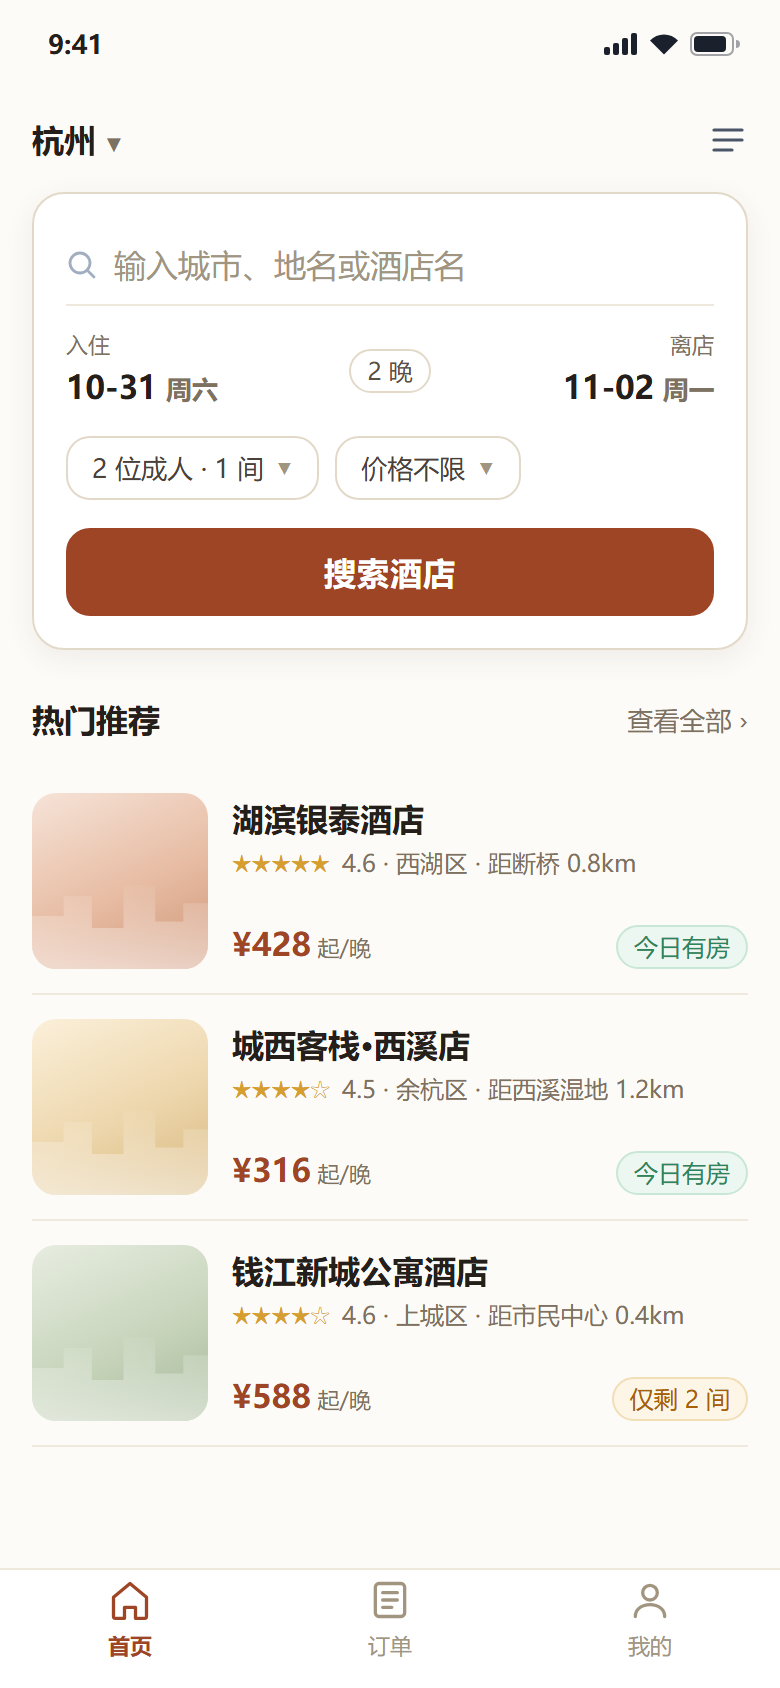
\includegraphics[width=\textwidth]{../UI界面/01_home_search.png}
  \caption{首页与搜索}
\end{subfigure}\hfill
\begin{subfigure}[b]{0.31\textwidth}
  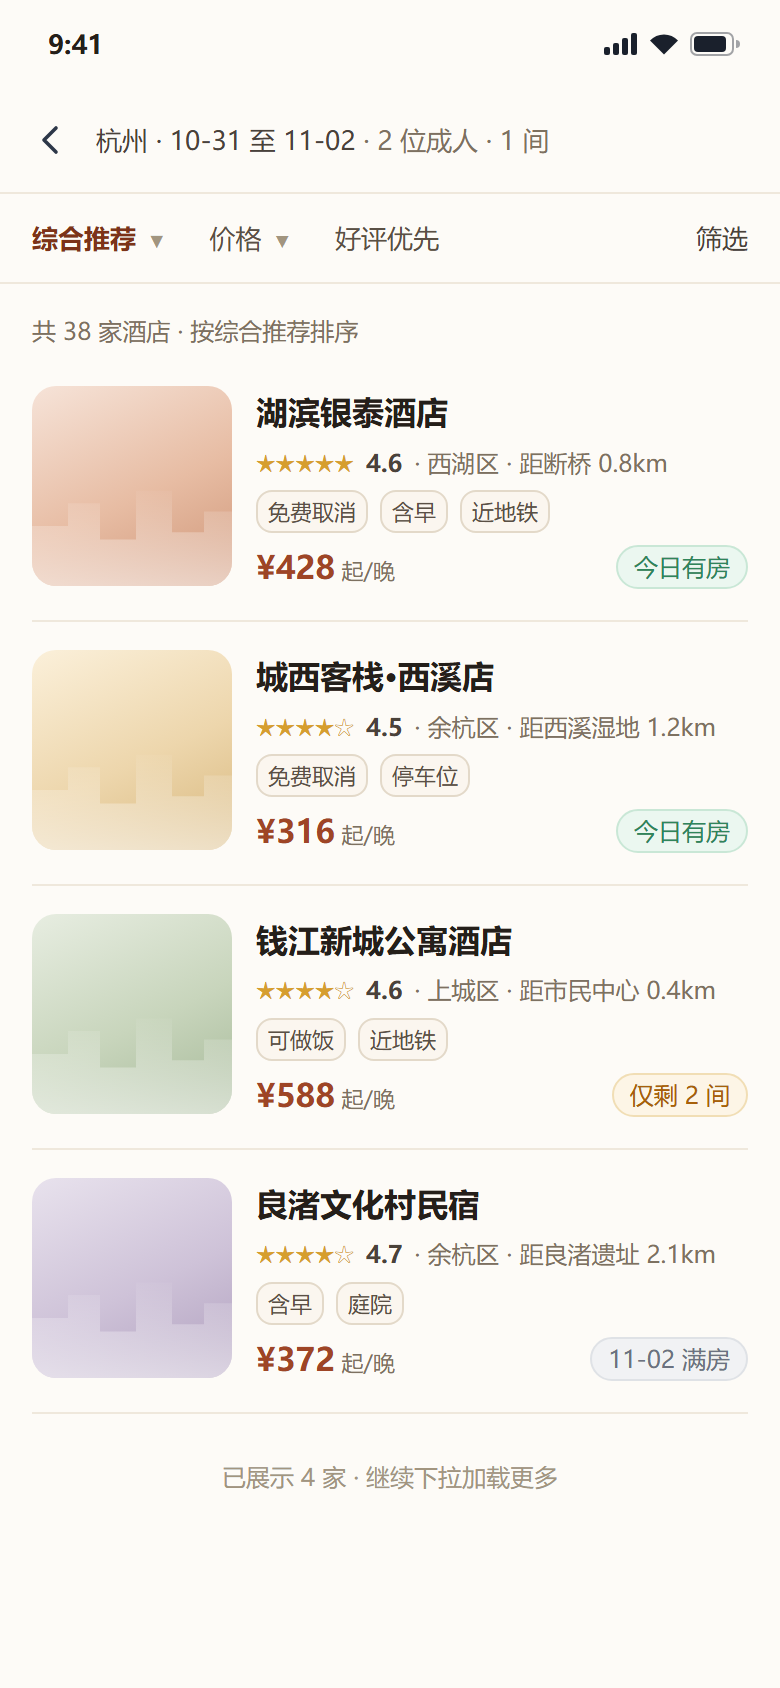
\includegraphics[width=\textwidth]{../UI界面/02_search_result.png}
  \caption{搜索结果}
\end{subfigure}\hfill
\begin{subfigure}[b]{0.31\textwidth}
  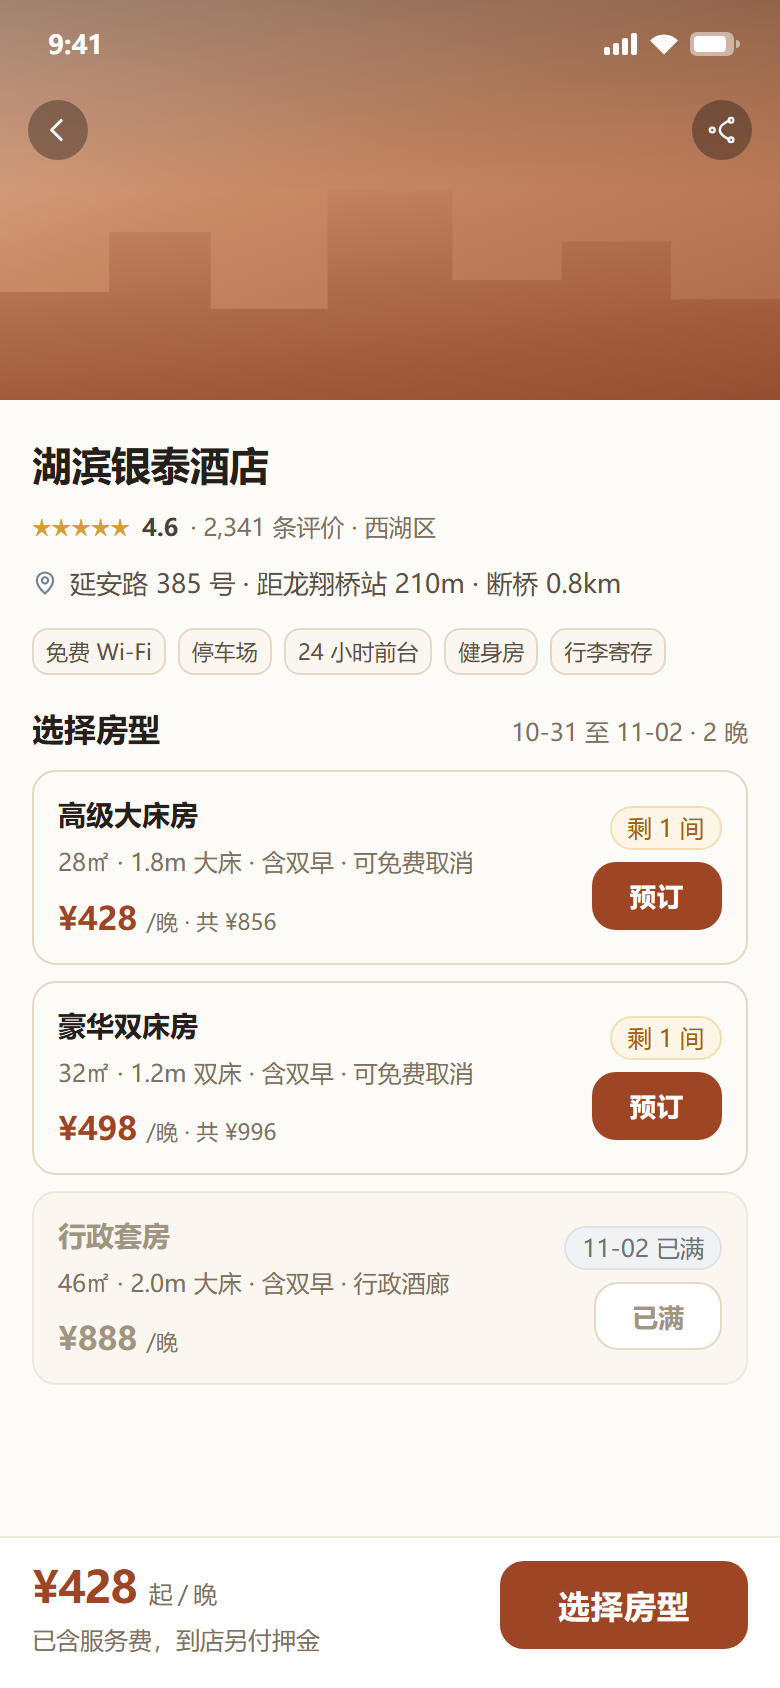
\includegraphics[width=\textwidth]{../UI界面/03_hotel_detail.png}
  \caption{酒店详情与房型}
\end{subfigure}
\caption{顾客端：搜索链路（01--03）}
\label{fig:ui_c1}
\end{figure}

\textbf{01 首页与搜索。} 展示城市、入住日期、离店日期、人数和价格条件，下方推荐门店并显示房量概况。房型的逐晚余量在详情页核对（REQ-002、REQ-013）。

\textbf{02 搜索结果。} 展示当前查询条件、排序筛选项及门店卡片；满房提示写明对应日期，避免将某一晚售罄误写成整店售罄（REQ-013）。

\textbf{03 酒店详情与房型选择。} 房型列表展示单价、总价和所选住期的可订量。示例包括：

\begin{itemize}
  \item 高级大床房 ¥428/晚 · 共 ¥856 · \textbf{剩 1 间}，可预订；
  \item 豪华双床房 ¥498/晚 · 共 ¥996 · \textbf{剩 1 间}，可预订；
  \item 行政套房 ¥888/晚 · \textbf{11-02 已满}，按钮置灰标注「已满」。
\end{itemize}

多晚可订量取各晚余量的最小值；行政套房有一晚售罄，因此不可提交两晚预订（REQ-013）。

\begin{figure}[htbp]
\centering
\begin{subfigure}[b]{0.31\textwidth}
  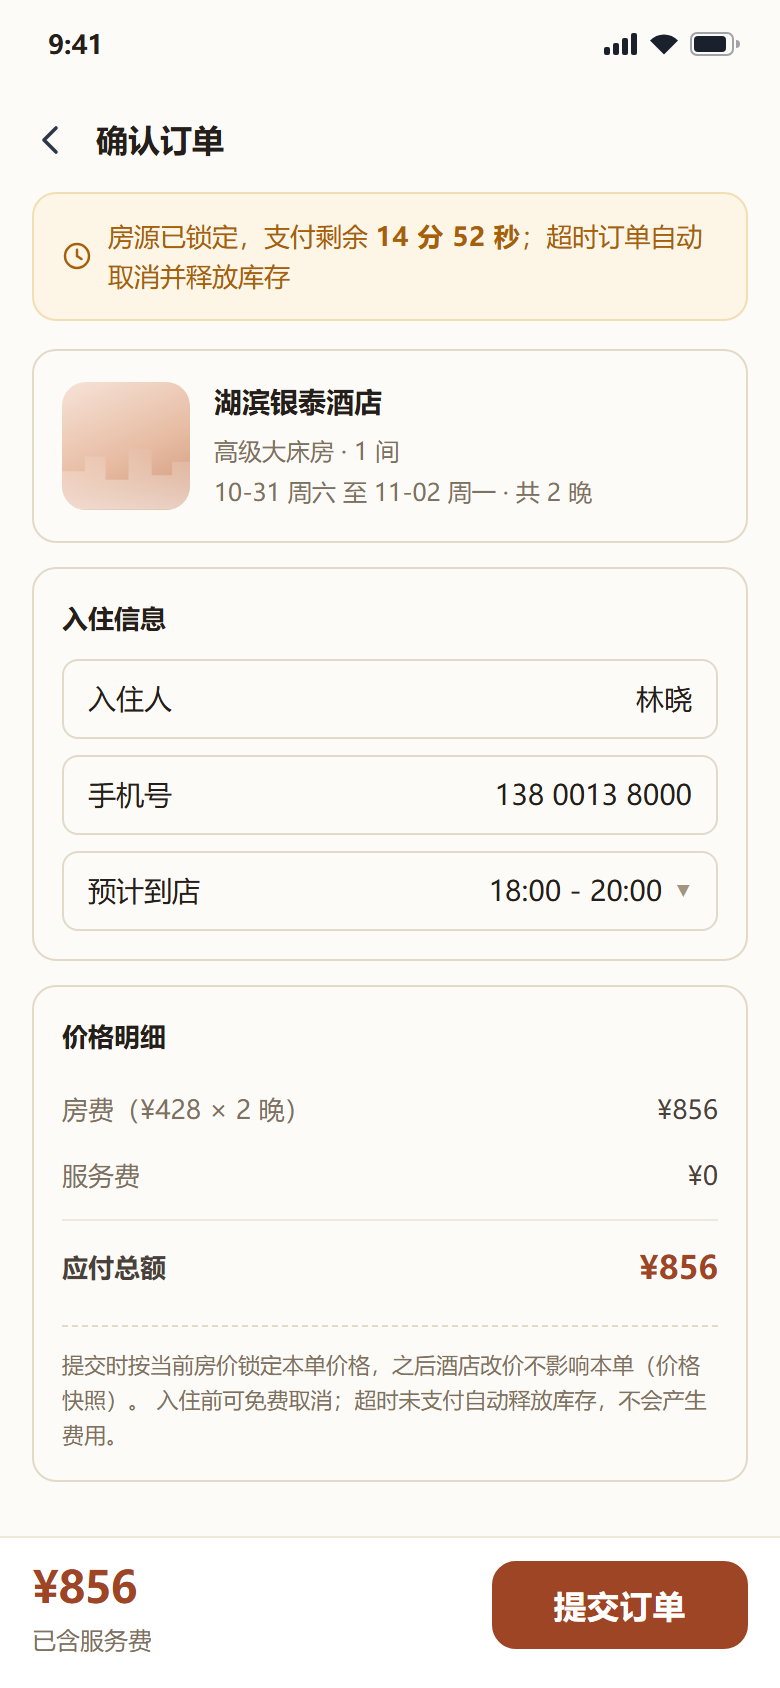
\includegraphics[width=\textwidth]{../UI界面/04_order_confirm.png}
  \caption{订单确认}
\end{subfigure}\hfill
\begin{subfigure}[b]{0.31\textwidth}
  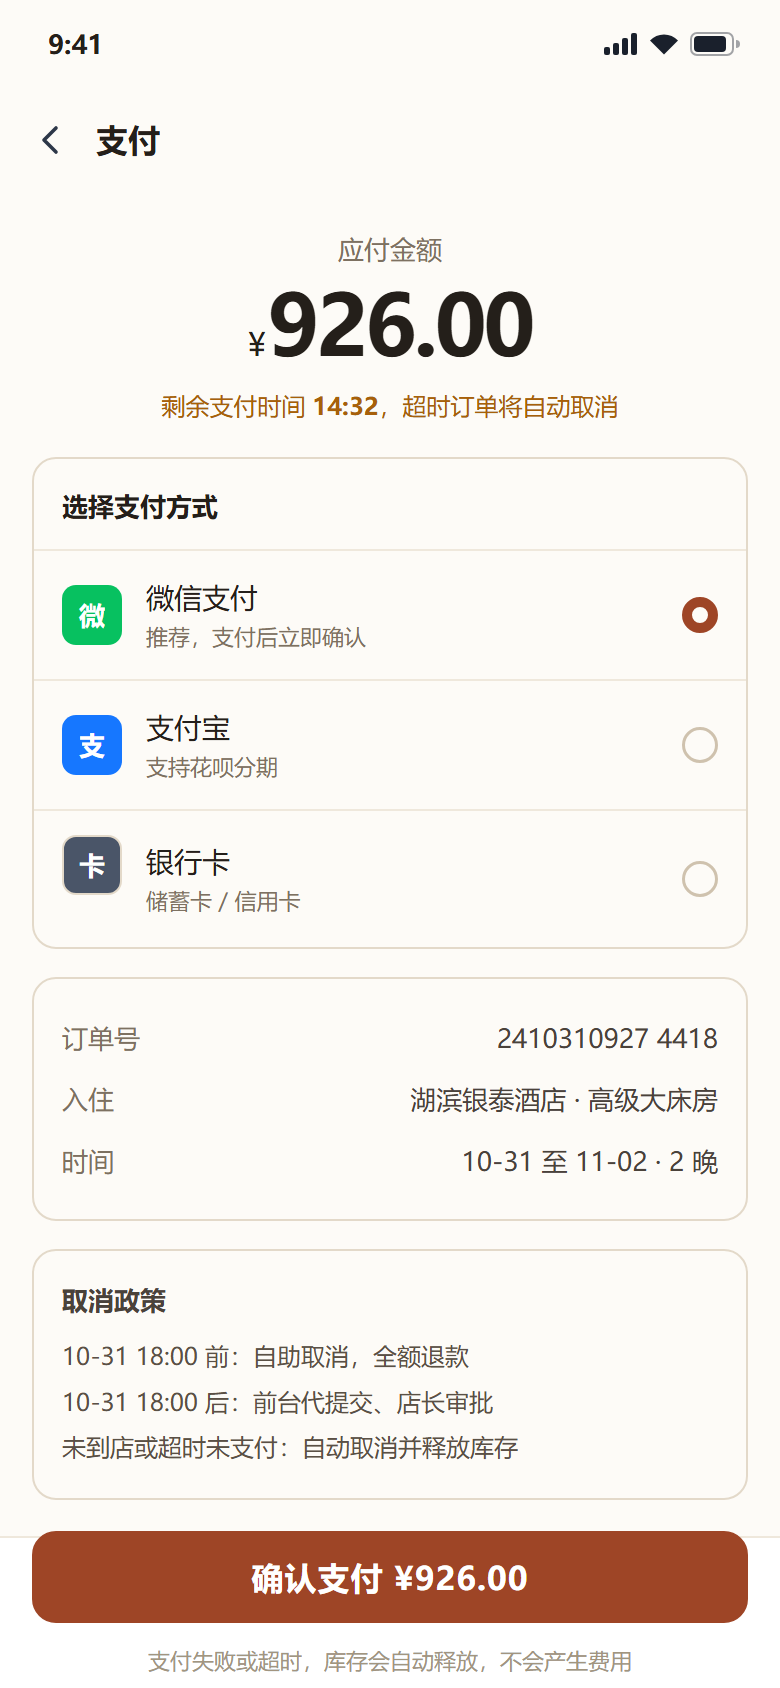
\includegraphics[width=\textwidth]{../UI界面/05_payment.png}
  \caption{支付}
\end{subfigure}\hfill
\begin{subfigure}[b]{0.31\textwidth}
  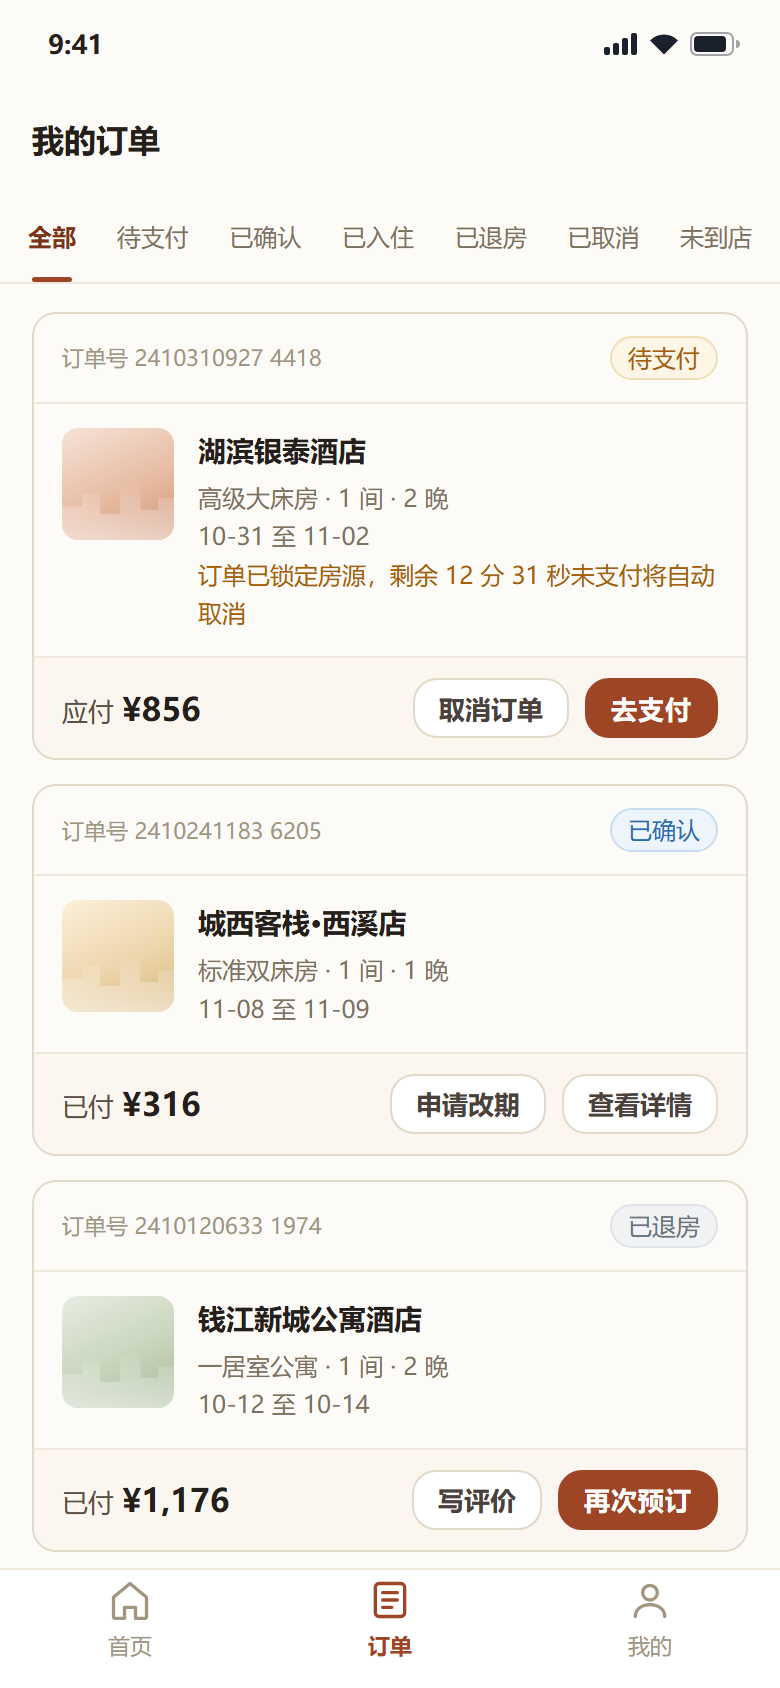
\includegraphics[width=\textwidth]{../UI界面/06_my_orders.png}
  \caption{我的订单}
\end{subfigure}
\caption{顾客端：确认、支付与订单（04--06）}
\label{fig:ui_c2}
\end{figure}

\textbf{04 订单确认。} 显示支付倒计时、入住人信息、价格明细和取消政策；超时未支付时取消订单并释放库存（REQ-020）。

示例订单为 ¥428 $\times$ 2 晚，共 ¥856；提交时将单价写入订单明细作为快照（REQ-023）。

\textbf{05 支付。} 展示应付金额、剩余支付时间、支付方式和取消政策：

\begin{itemize}
  \item 10-31 18:00 前：自助取消，全额退款（REQ-021 前段）；
  \item 10-31 18:00 后：前台代提交、店长审批（REQ-021 后段）；
  \item 未到店或超时未支付：自动取消并释放库存（REQ-020、REQ-022）。
\end{itemize}


\textbf{06 我的订单。} 支持按订单状态筛选。示例卡片提供以下操作：

\begin{itemize}
  \item 待支付：取消订单、去支付，并显示剩余支付时间；
  \item 已确认：申请改期、查看详情；
  \item 已退房：写评价、再次预订（REQ-003）。
\end{itemize}


\begin{figure}[htbp]
\centering
\begin{subfigure}[b]{0.34\textwidth}
  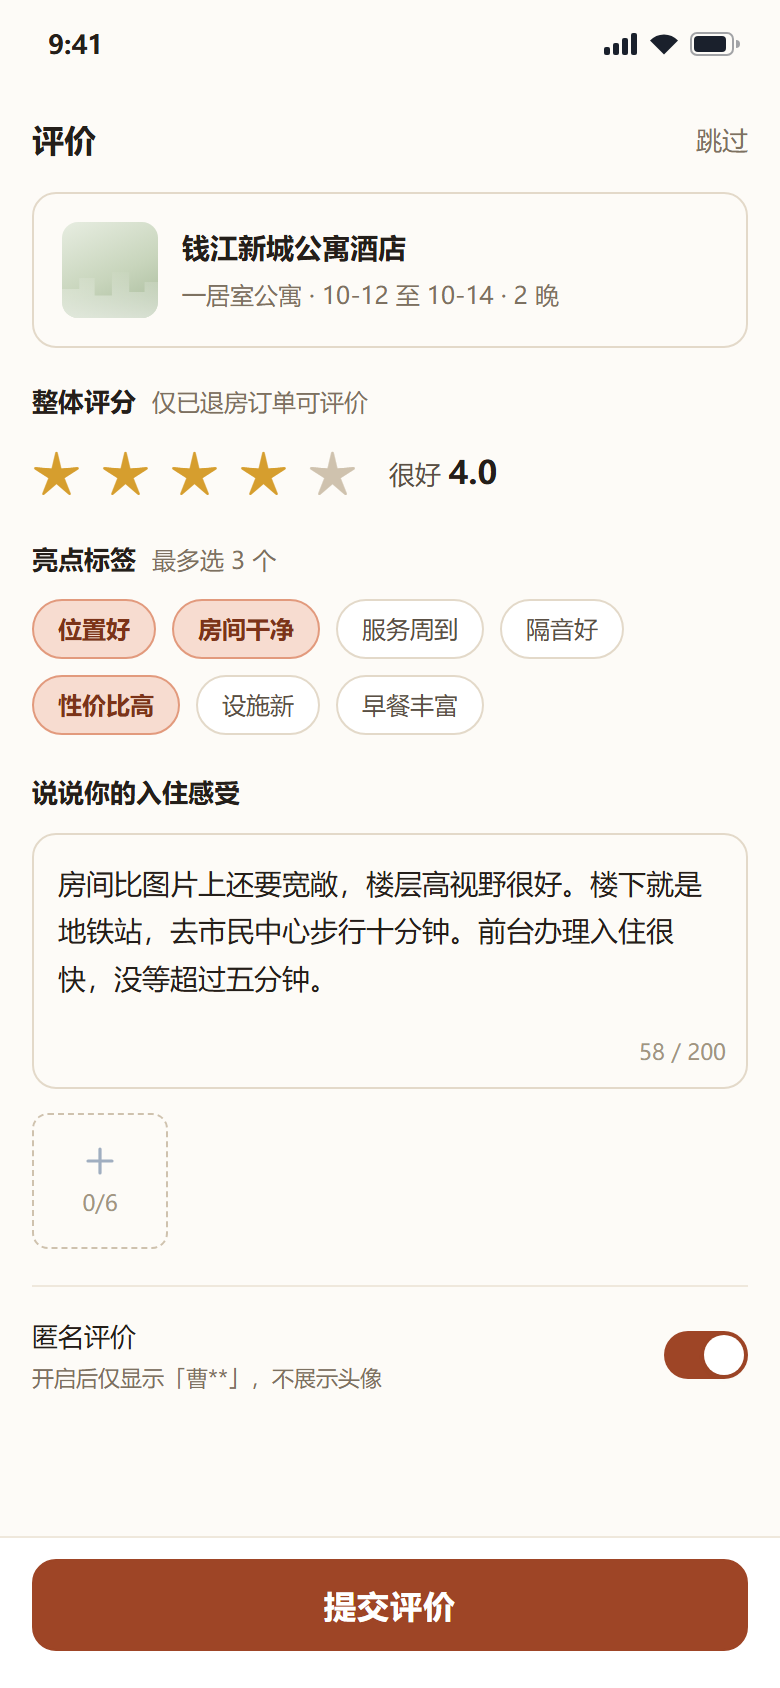
\includegraphics[width=\textwidth]{../UI界面/07_review_submit.png}
  \caption{评价提交}
\end{subfigure}
\caption{顾客端：评价提交（07）}
\label{fig:ui_c3}
\end{figure}

\textbf{07 评价提交。} 仅向已退房订单开放，包含评分、最多三个标签、200 字以内的文字和匿名选项（REQ-003）。

\subsection{前台端（4 屏，桌面工作台）}

前台端按房态、入住、退房和线下开单分为四屏。

\begin{figure}[htbp]
\centering
\begin{subfigure}[b]{0.95\textwidth}
  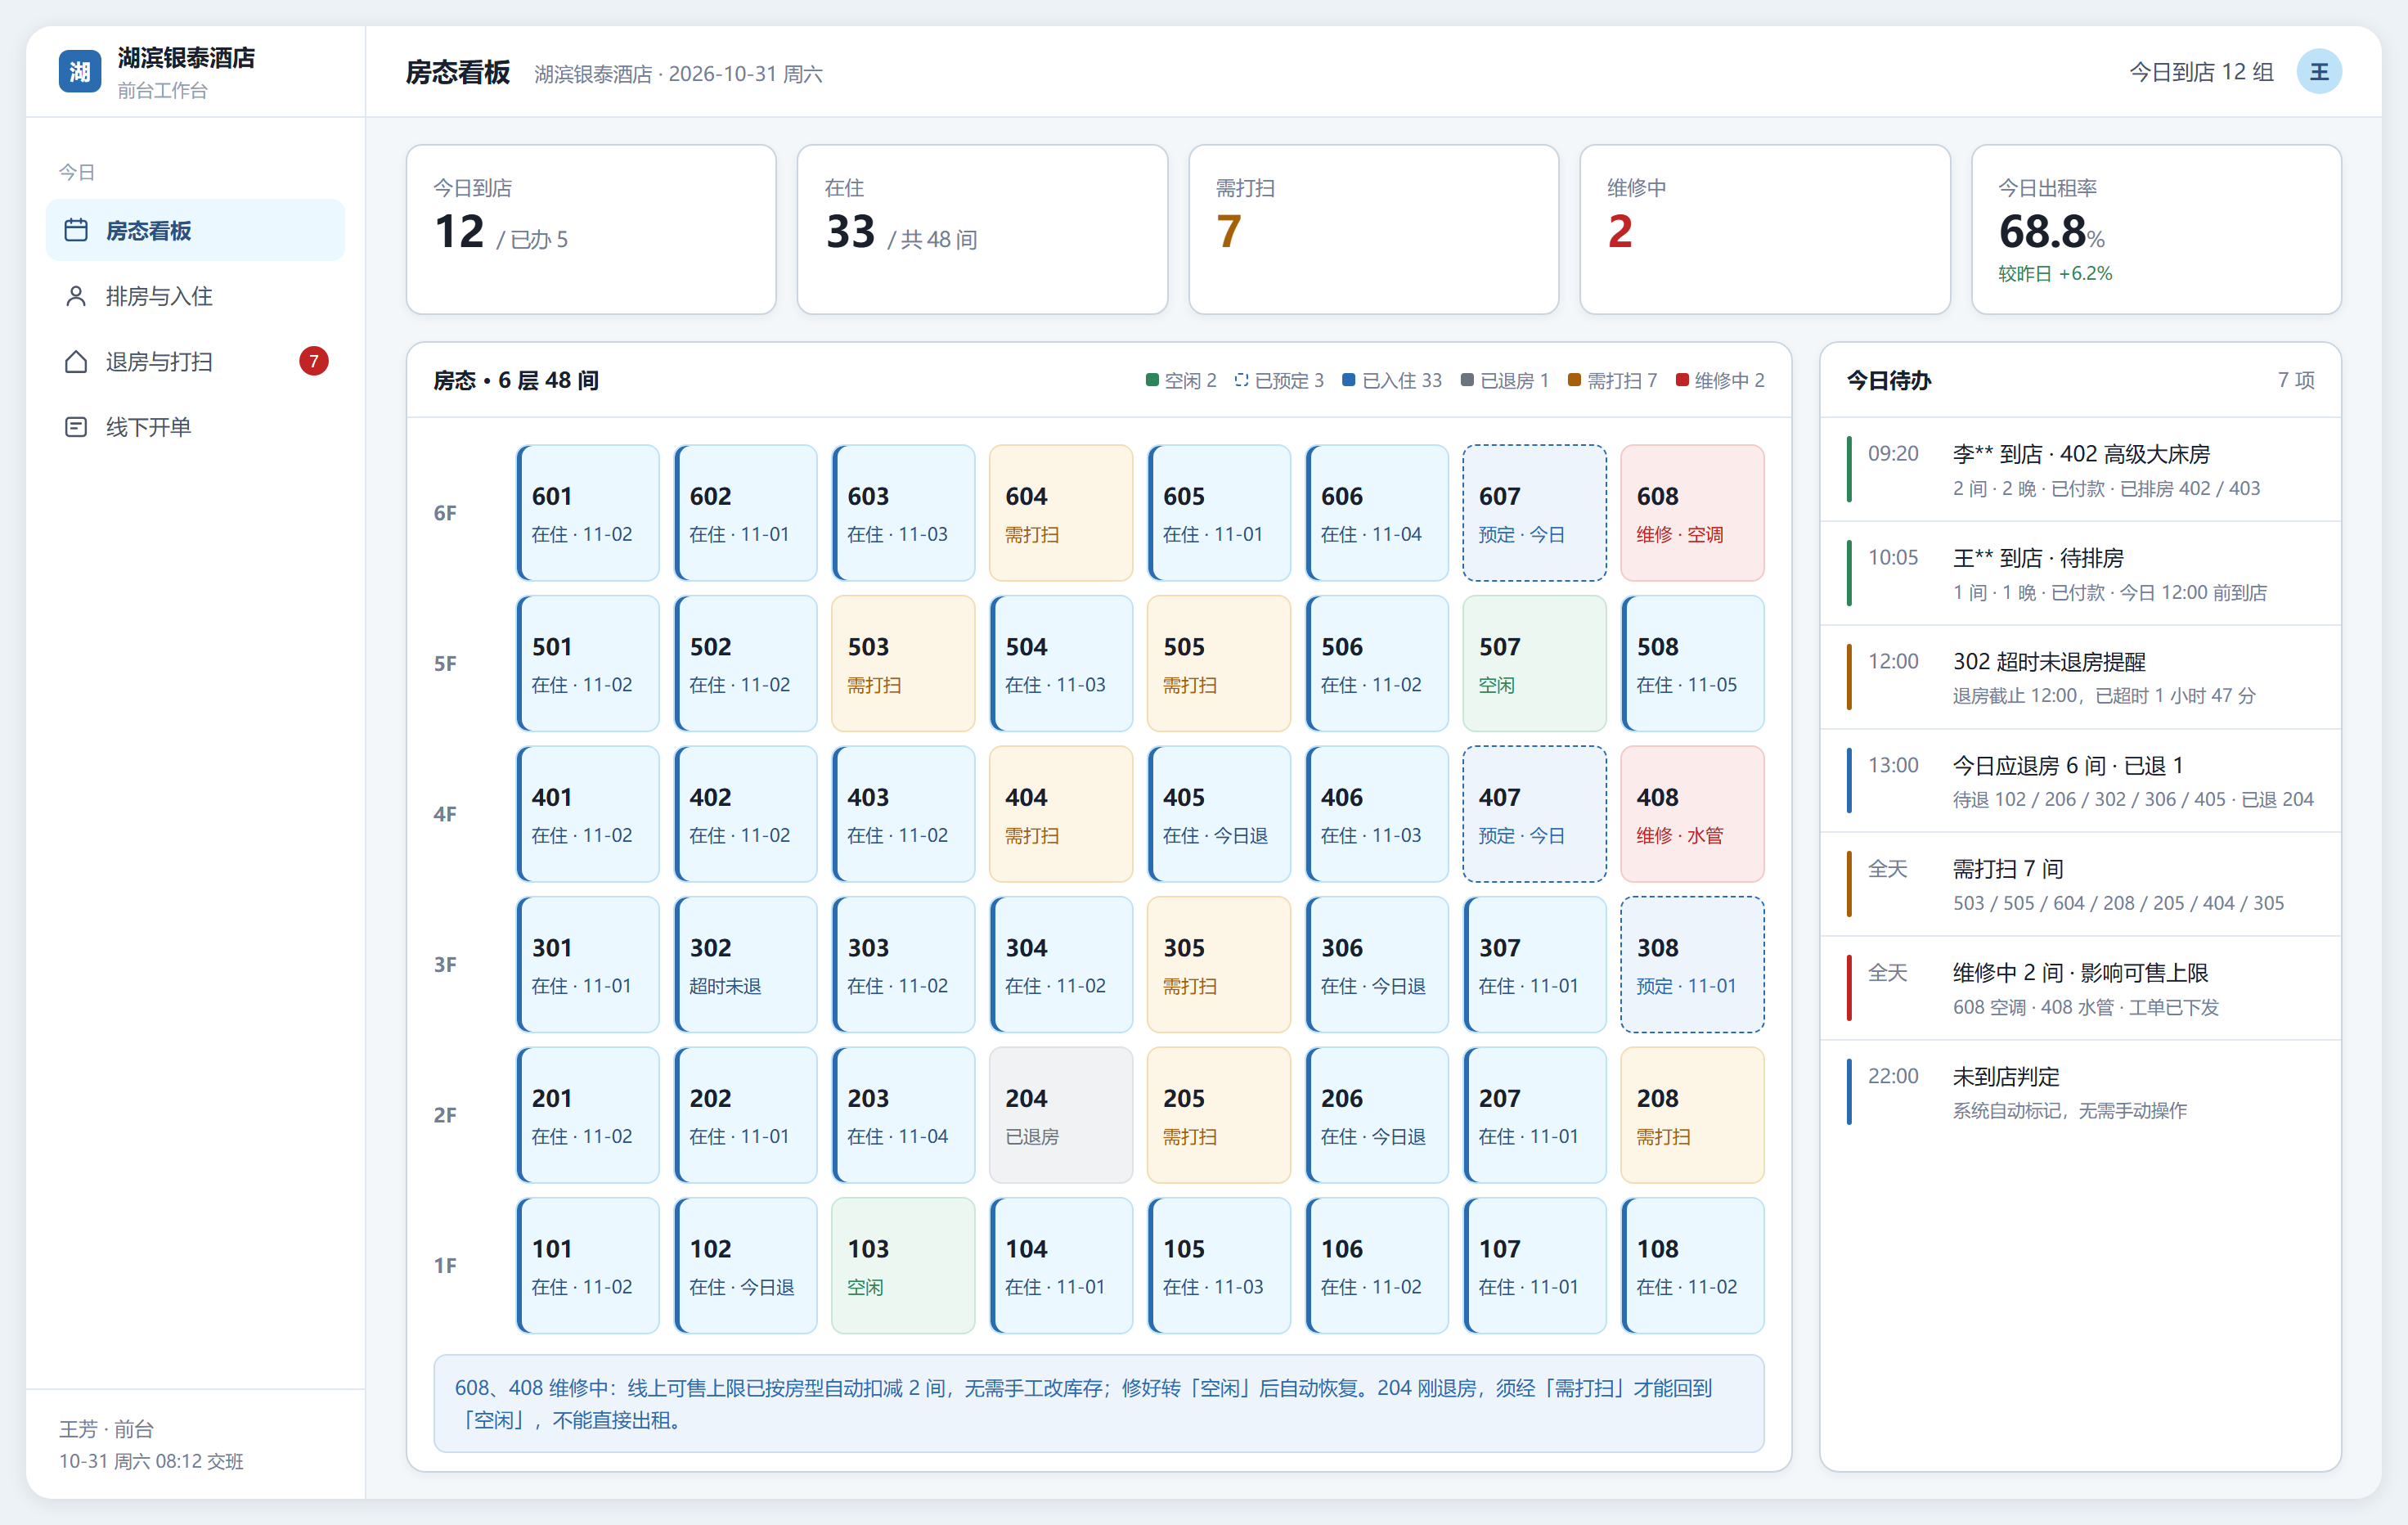
\includegraphics[width=\textwidth]{../UI界面/08_room_board.png}
  \caption{房态看板与今日待办}
\end{subfigure}\\[3pt]
\begin{subfigure}[b]{0.95\textwidth}
  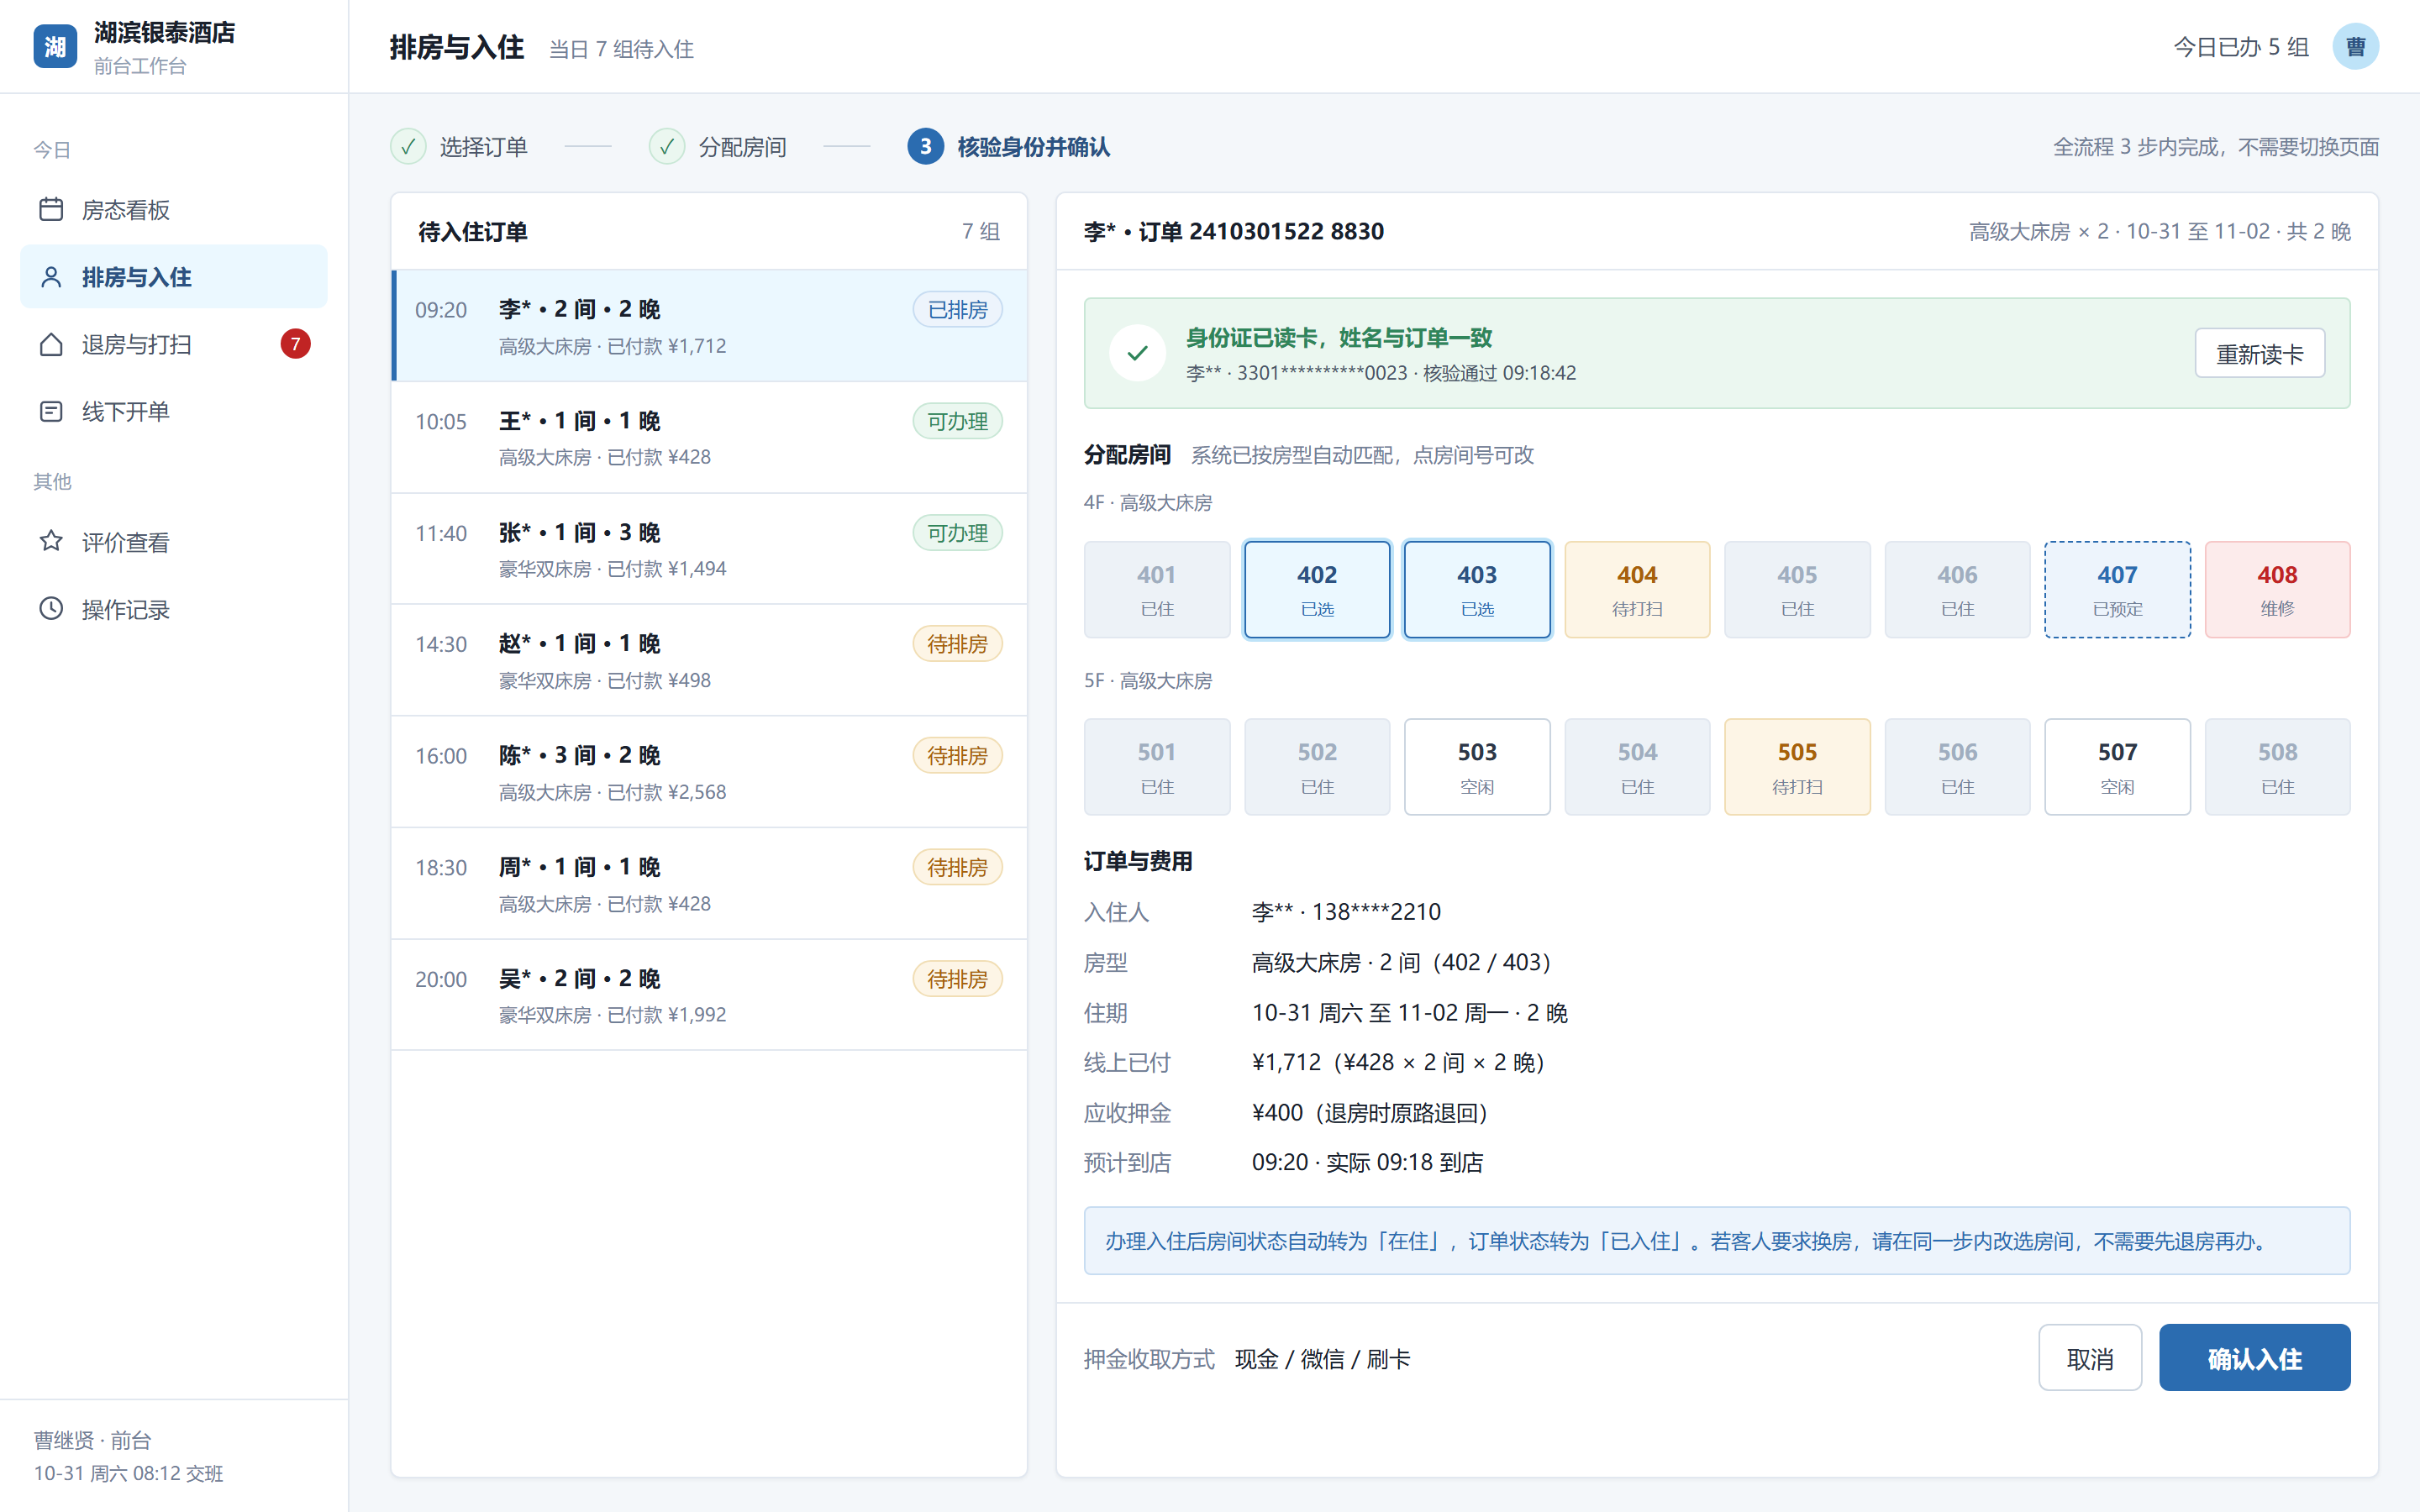
\includegraphics[width=\textwidth]{../UI界面/09_checkin.png}
  \caption{排房与入住办理}
\end{subfigure}
\caption{前台端：房态看板与入住（08--09）}
\label{fig:ui_f1}
\end{figure}

\textbf{08 房态看板。} 按楼层显示 48 间房的六种房态，并汇总在住 33 间、需打扫 7 间、维修中 2 间。超时未退和维修房间单独标示；维修数用于计算日库存上限（REQ-005、REQ-022、REQ-034）。

\textbf{09 排房与入住。} 依次选择订单、分配房间、核验身份并确认，控制在三步内（REQ-018）。系统提供建议房号，前台可改选；维修中、已入住、已预定及待打扫的房间不可选（REQ-024）。

\begin{figure}[htbp]
\centering
\begin{subfigure}[b]{0.95\textwidth}
  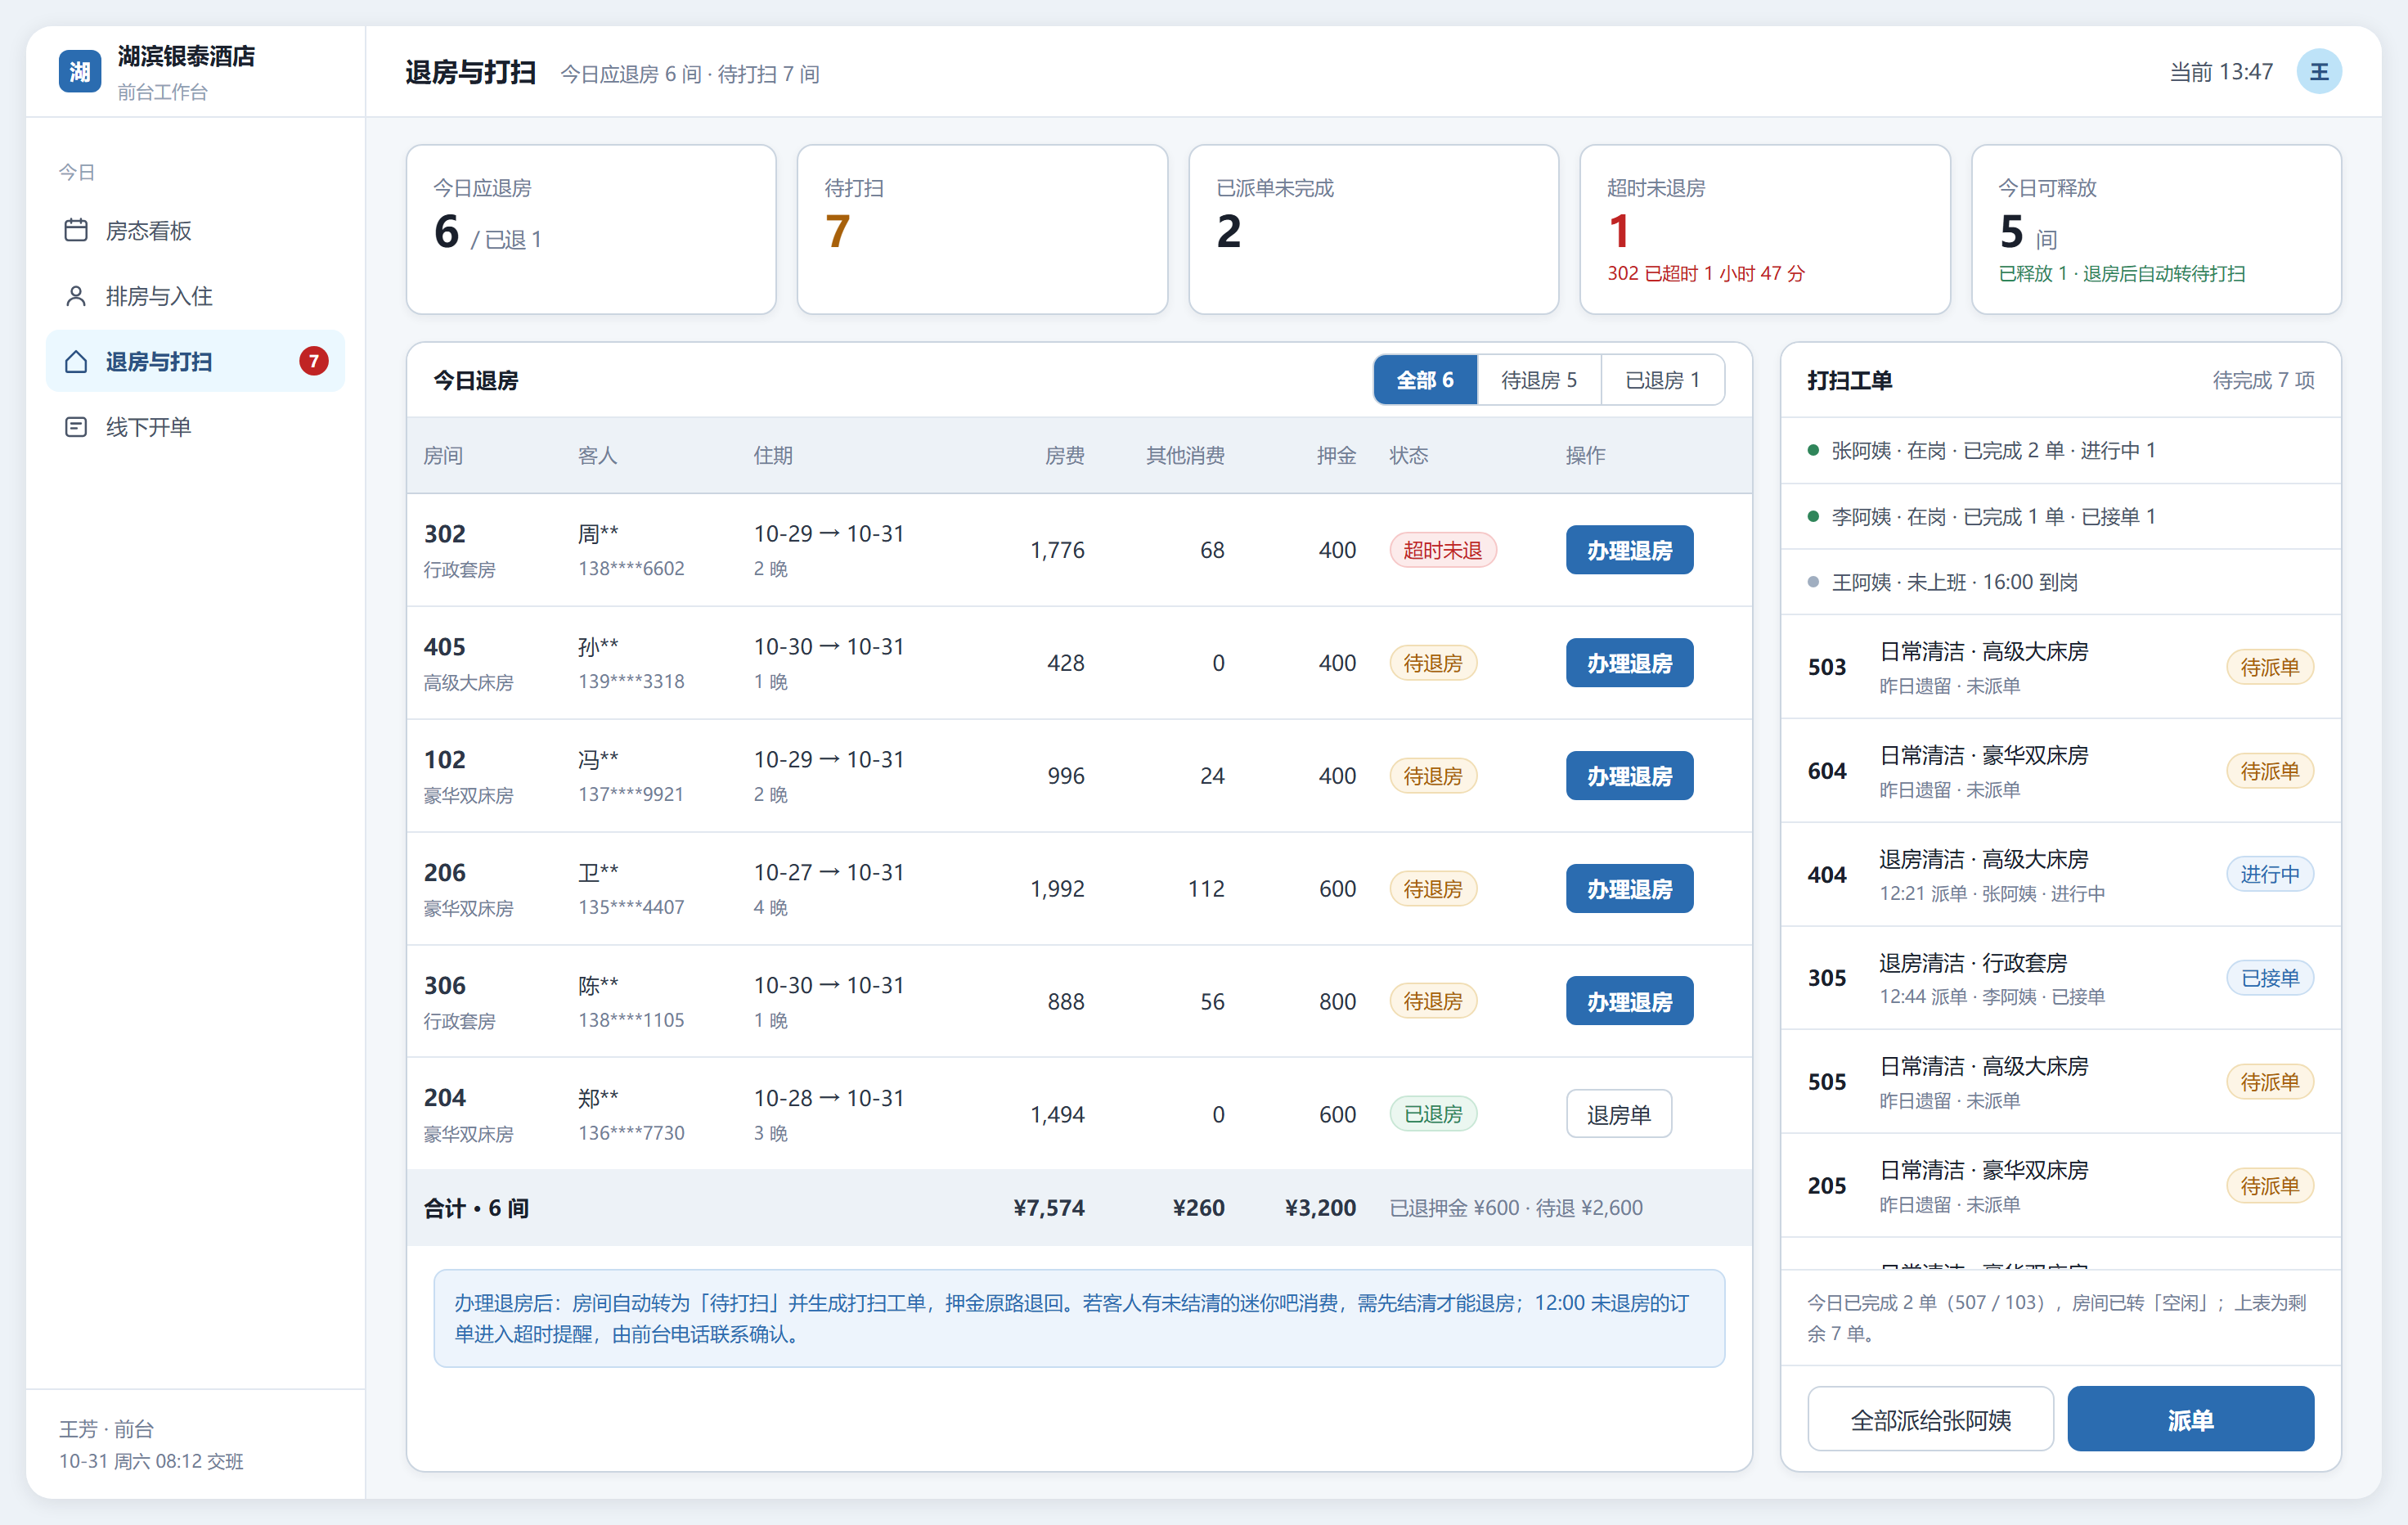
\includegraphics[width=\textwidth]{../UI界面/10_housekeeping.png}
  \caption{退房与打扫}
\end{subfigure}\\[3pt]
\begin{subfigure}[b]{0.95\textwidth}
  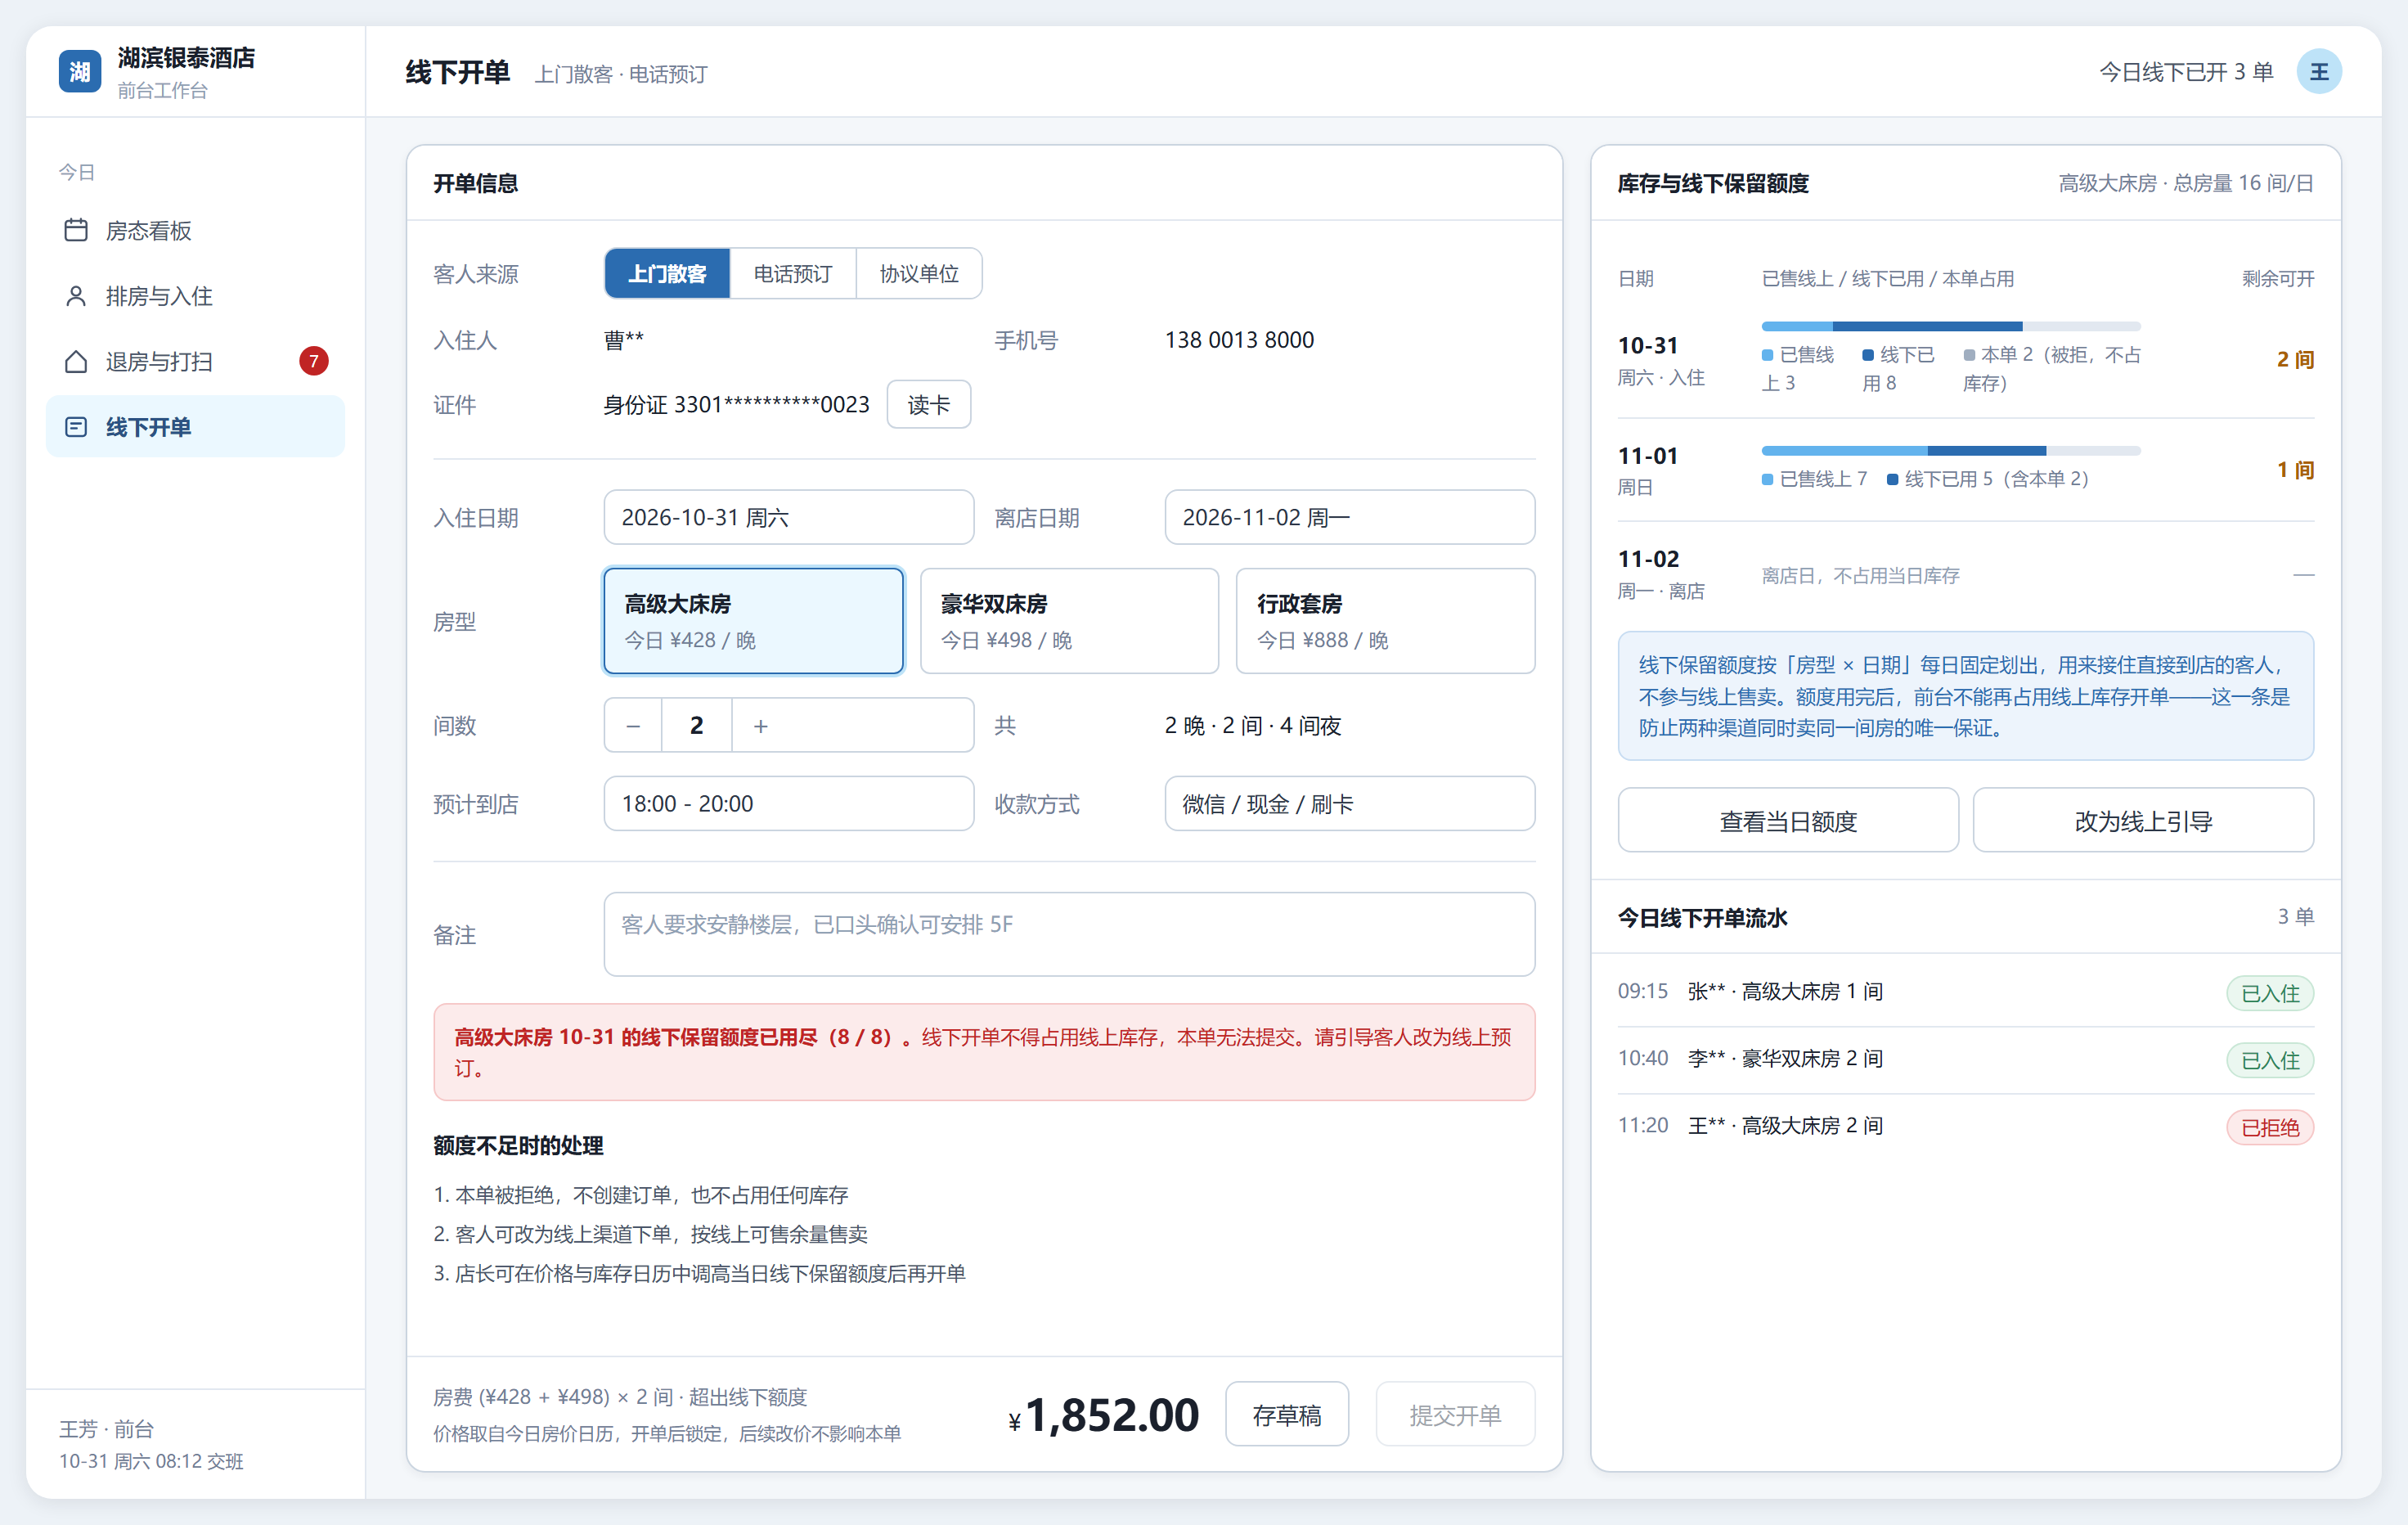
\includegraphics[width=\textwidth]{../UI界面/11_walkin_order.png}
  \caption{线下开单与库存校验}
\end{subfigure}
\caption{前台端：退房与线下开单（10--11）}
\label{fig:ui_f2}
\end{figure}

\textbf{10 退房与打扫。} 列出应退房、已退房、待打扫与超时未退房记录；每行可直接办理退房并派发打扫工单。房费、其他消费和押金分列，供退房结算使用（REQ-003、REQ-025）。

\textbf{11 线下开单。} 前台填写入住人、住期、房型、间数和收款方式；系统逐晚展示线上已售、线下已用和剩余可开量。线下保留额度不足时，界面提示：

\begin{quote}
\zihao{5}高级大床房 10-31 的线下保留额度已用尽（8 / 8）。继续开单将占用线上可售库存，可能造成线上超卖。请改为引导客人线上预订，或提交店长审批后再开单。
\end{quote}

超额开单提交后进入待审批状态，审批通过前不占库存；批准后重新校验并扣减库存，不足则开单失败。成功开单后生成排房任务（REQ-033）。

\subsection{店长端（4 屏，桌面后台）}

店长端提供定价、审批、排班评价和消息查询四项主要入口。

\begin{figure}[htbp]
\centering
\begin{subfigure}[b]{0.95\textwidth}
  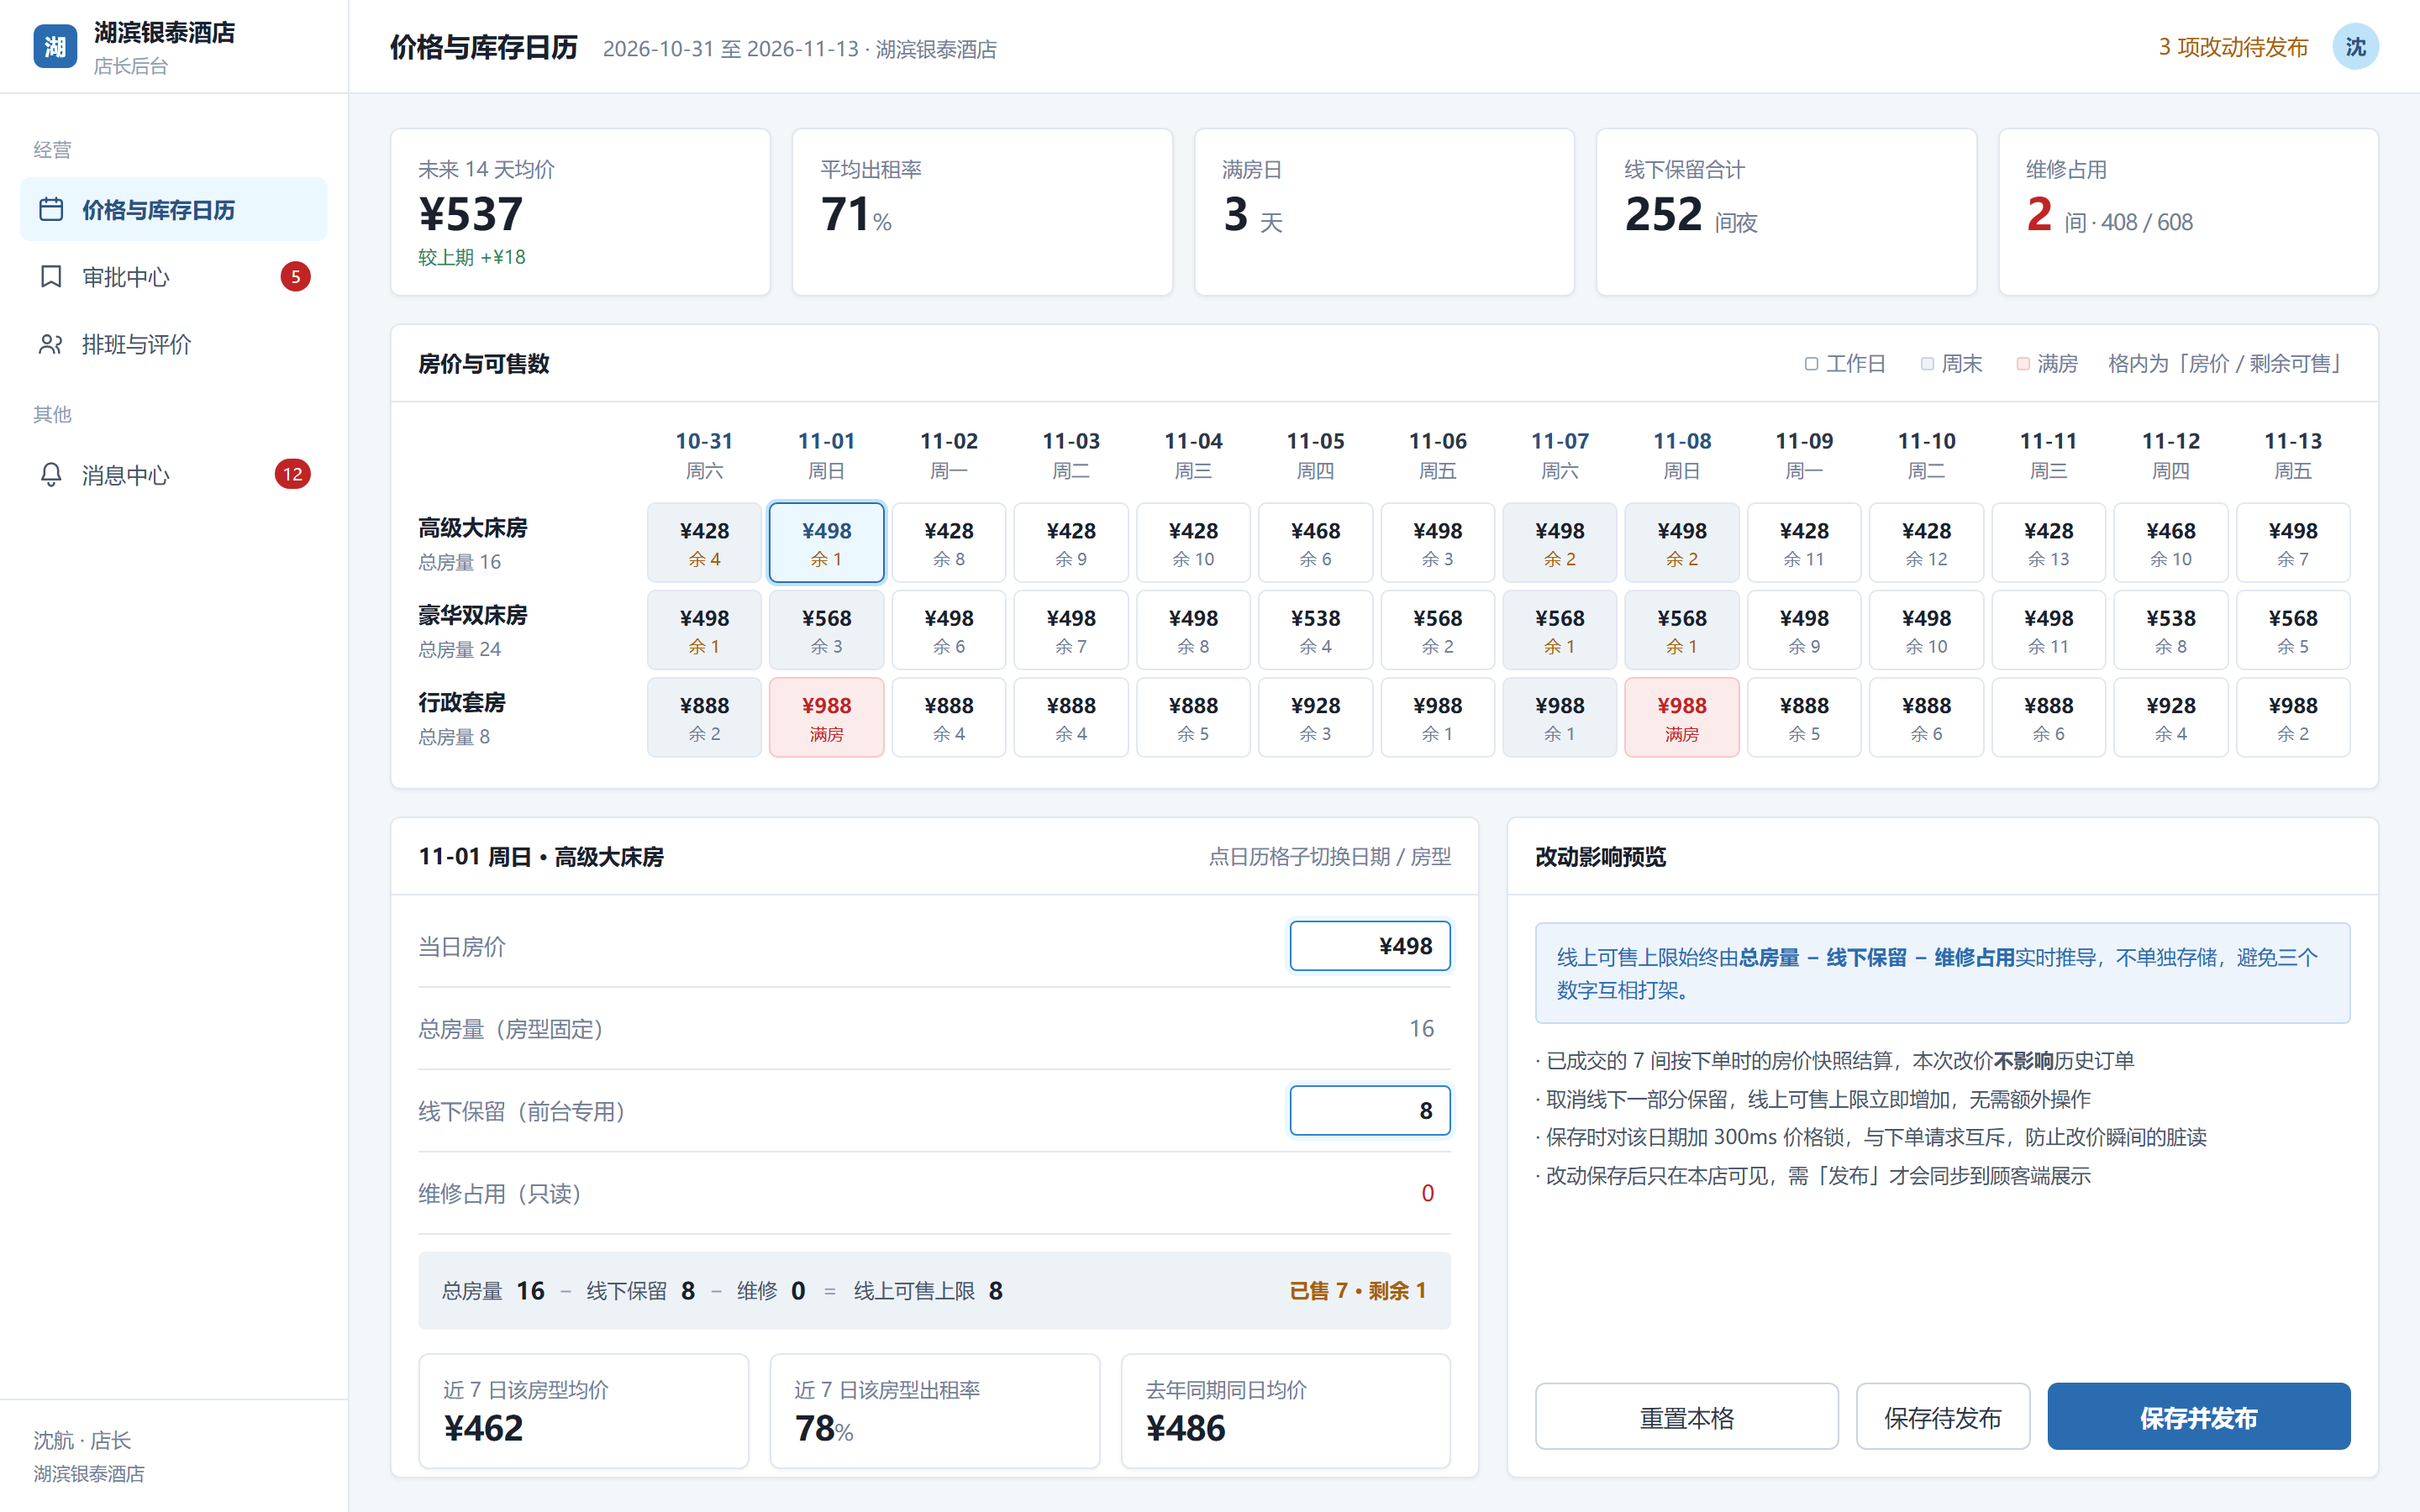
\includegraphics[width=\textwidth]{../UI界面/12_price_calendar.png}
  \caption{价格与库存日历}
\end{subfigure}\\[3pt]
\begin{subfigure}[b]{0.95\textwidth}
  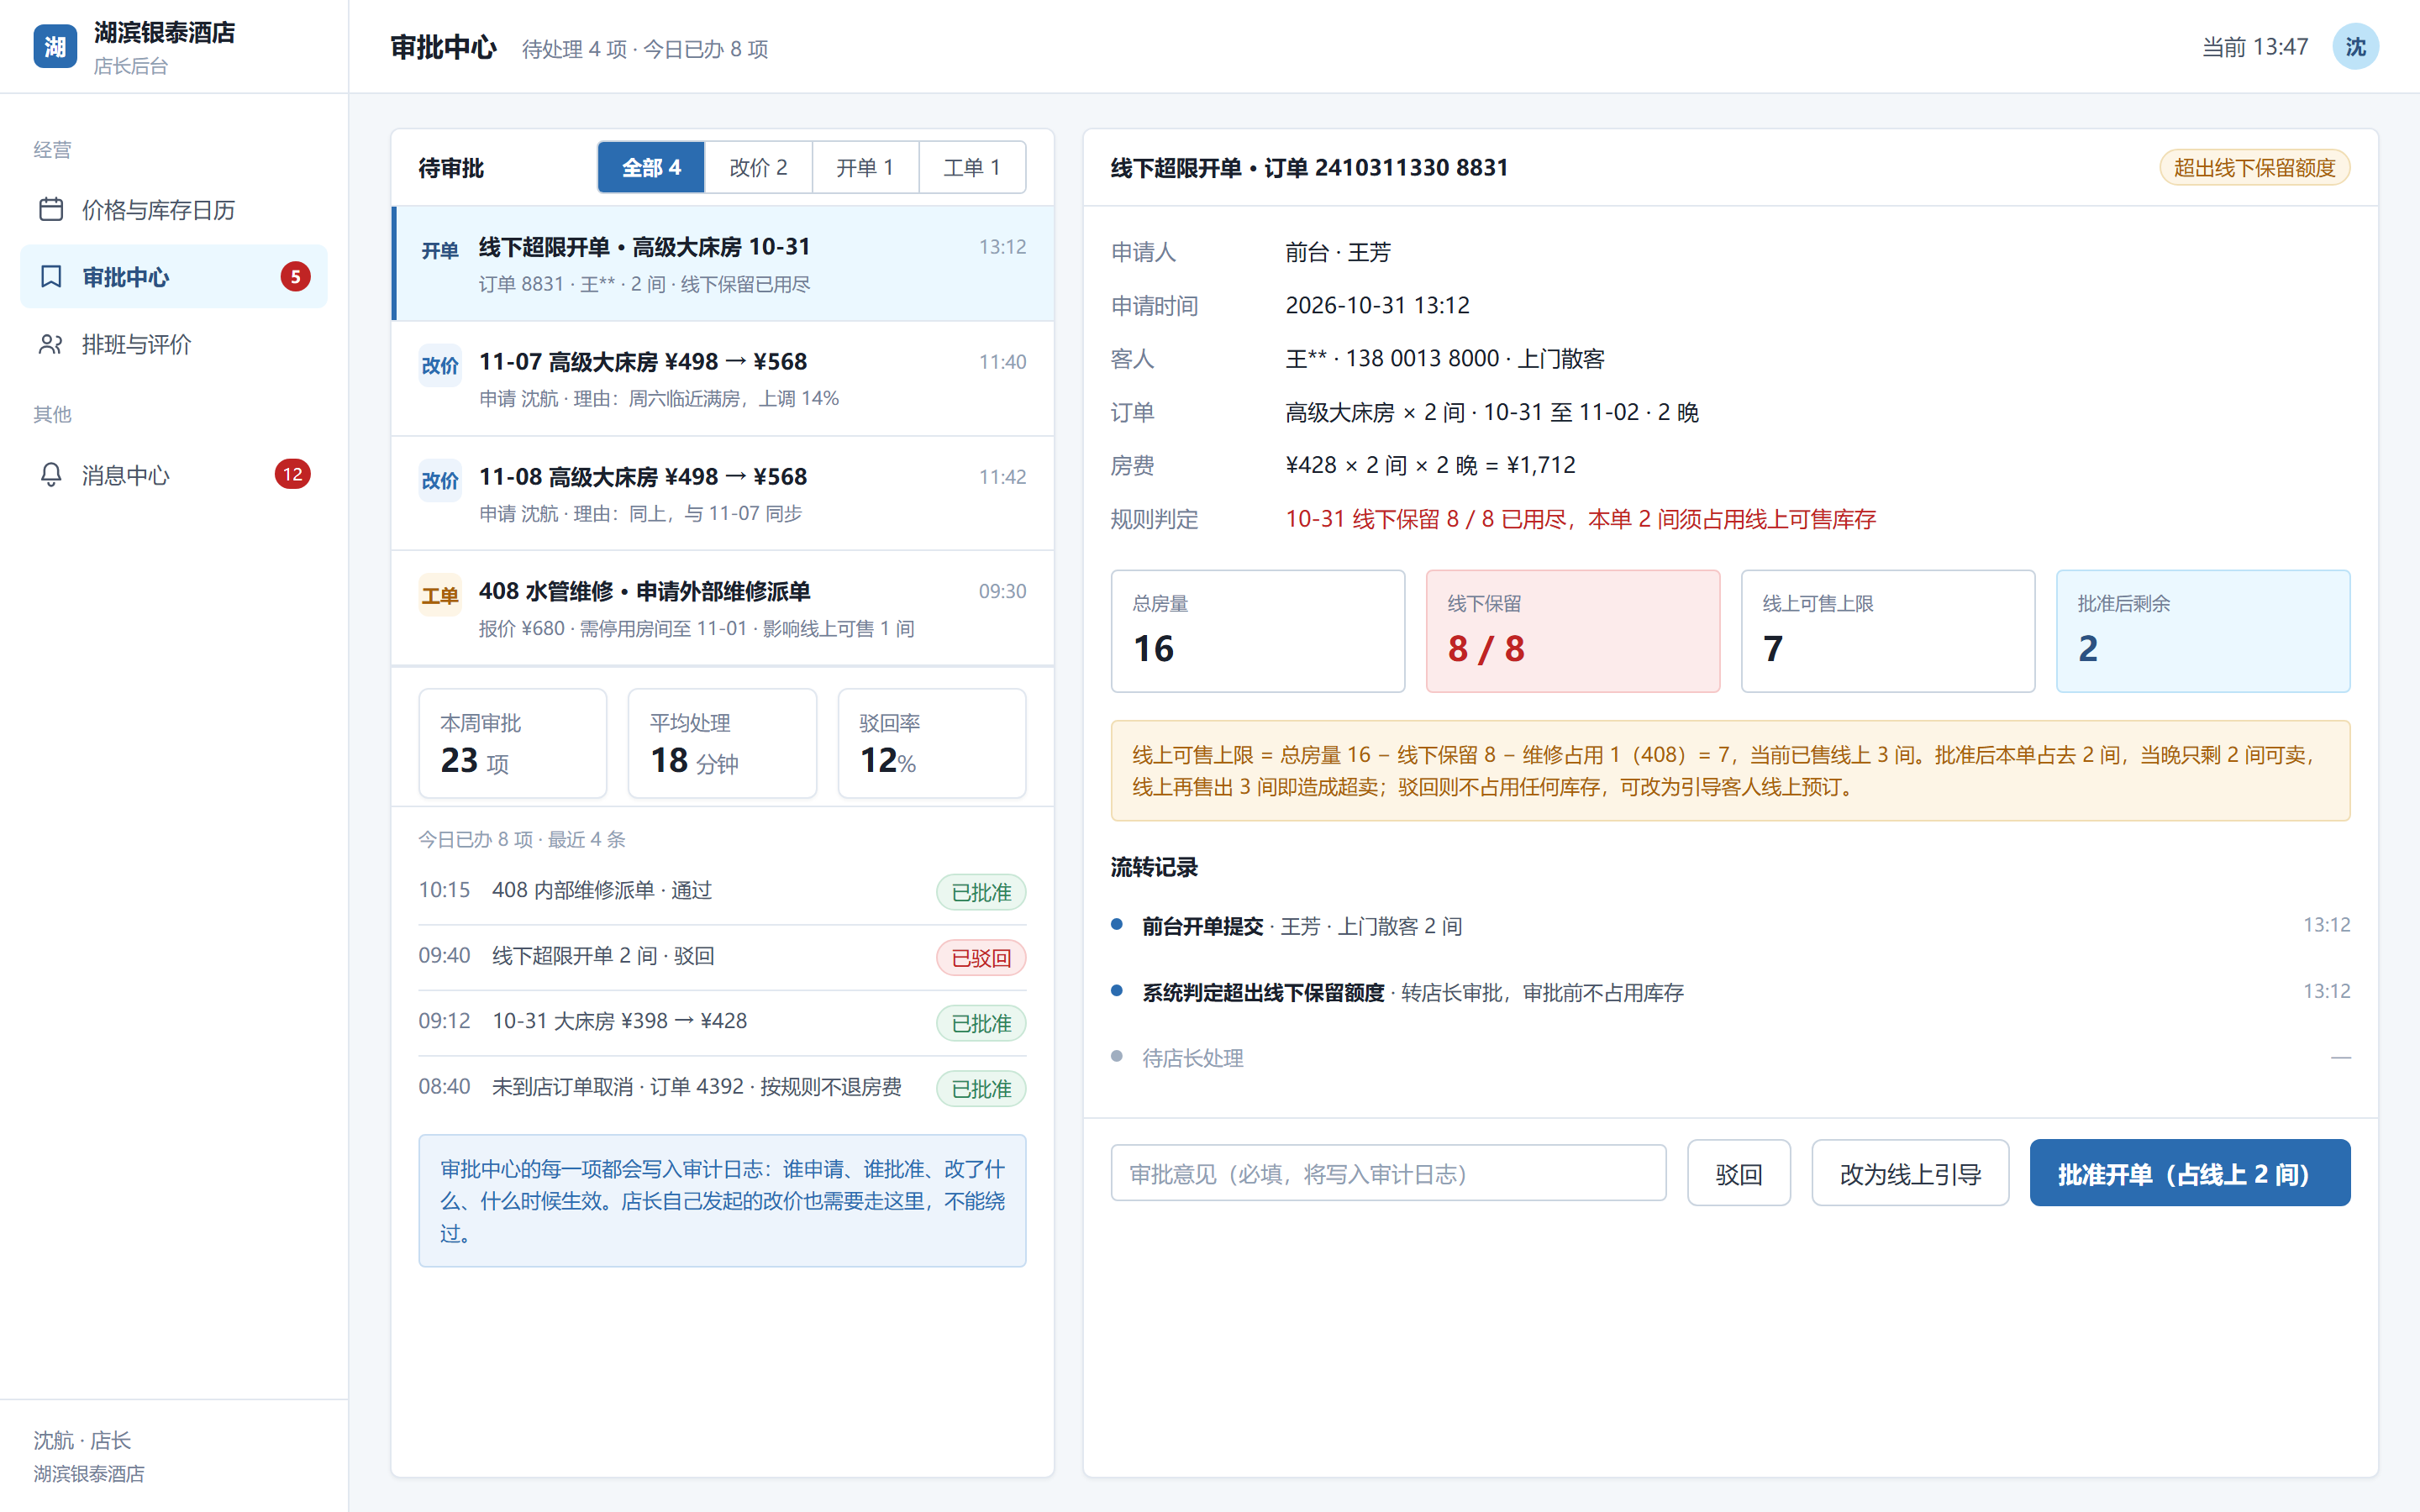
\includegraphics[width=\textwidth]{../UI界面/13_approval_center.png}
  \caption{审批中心}
\end{subfigure}
\caption{店长端：定价与审批（12--13）}
\label{fig:ui_m1}
\end{figure}

\textbf{12 价格与库存日历。} 按房型与日期展示未来 14 天日价、线上余量和线下保留额度；店长可调整价格与可售上限。维修占用与待发布修改单独汇总（REQ-006、REQ-013、REQ-033）。

\textbf{13 审批中心。} 按改价、超限开单和工单类型列出待办；选中申请后展示金额、库存影响及申请理由。审批意见必填，批准或驳回均记录审计日志（REQ-014）。

\begin{figure}[htbp]
\centering
\begin{subfigure}[b]{0.95\textwidth}
  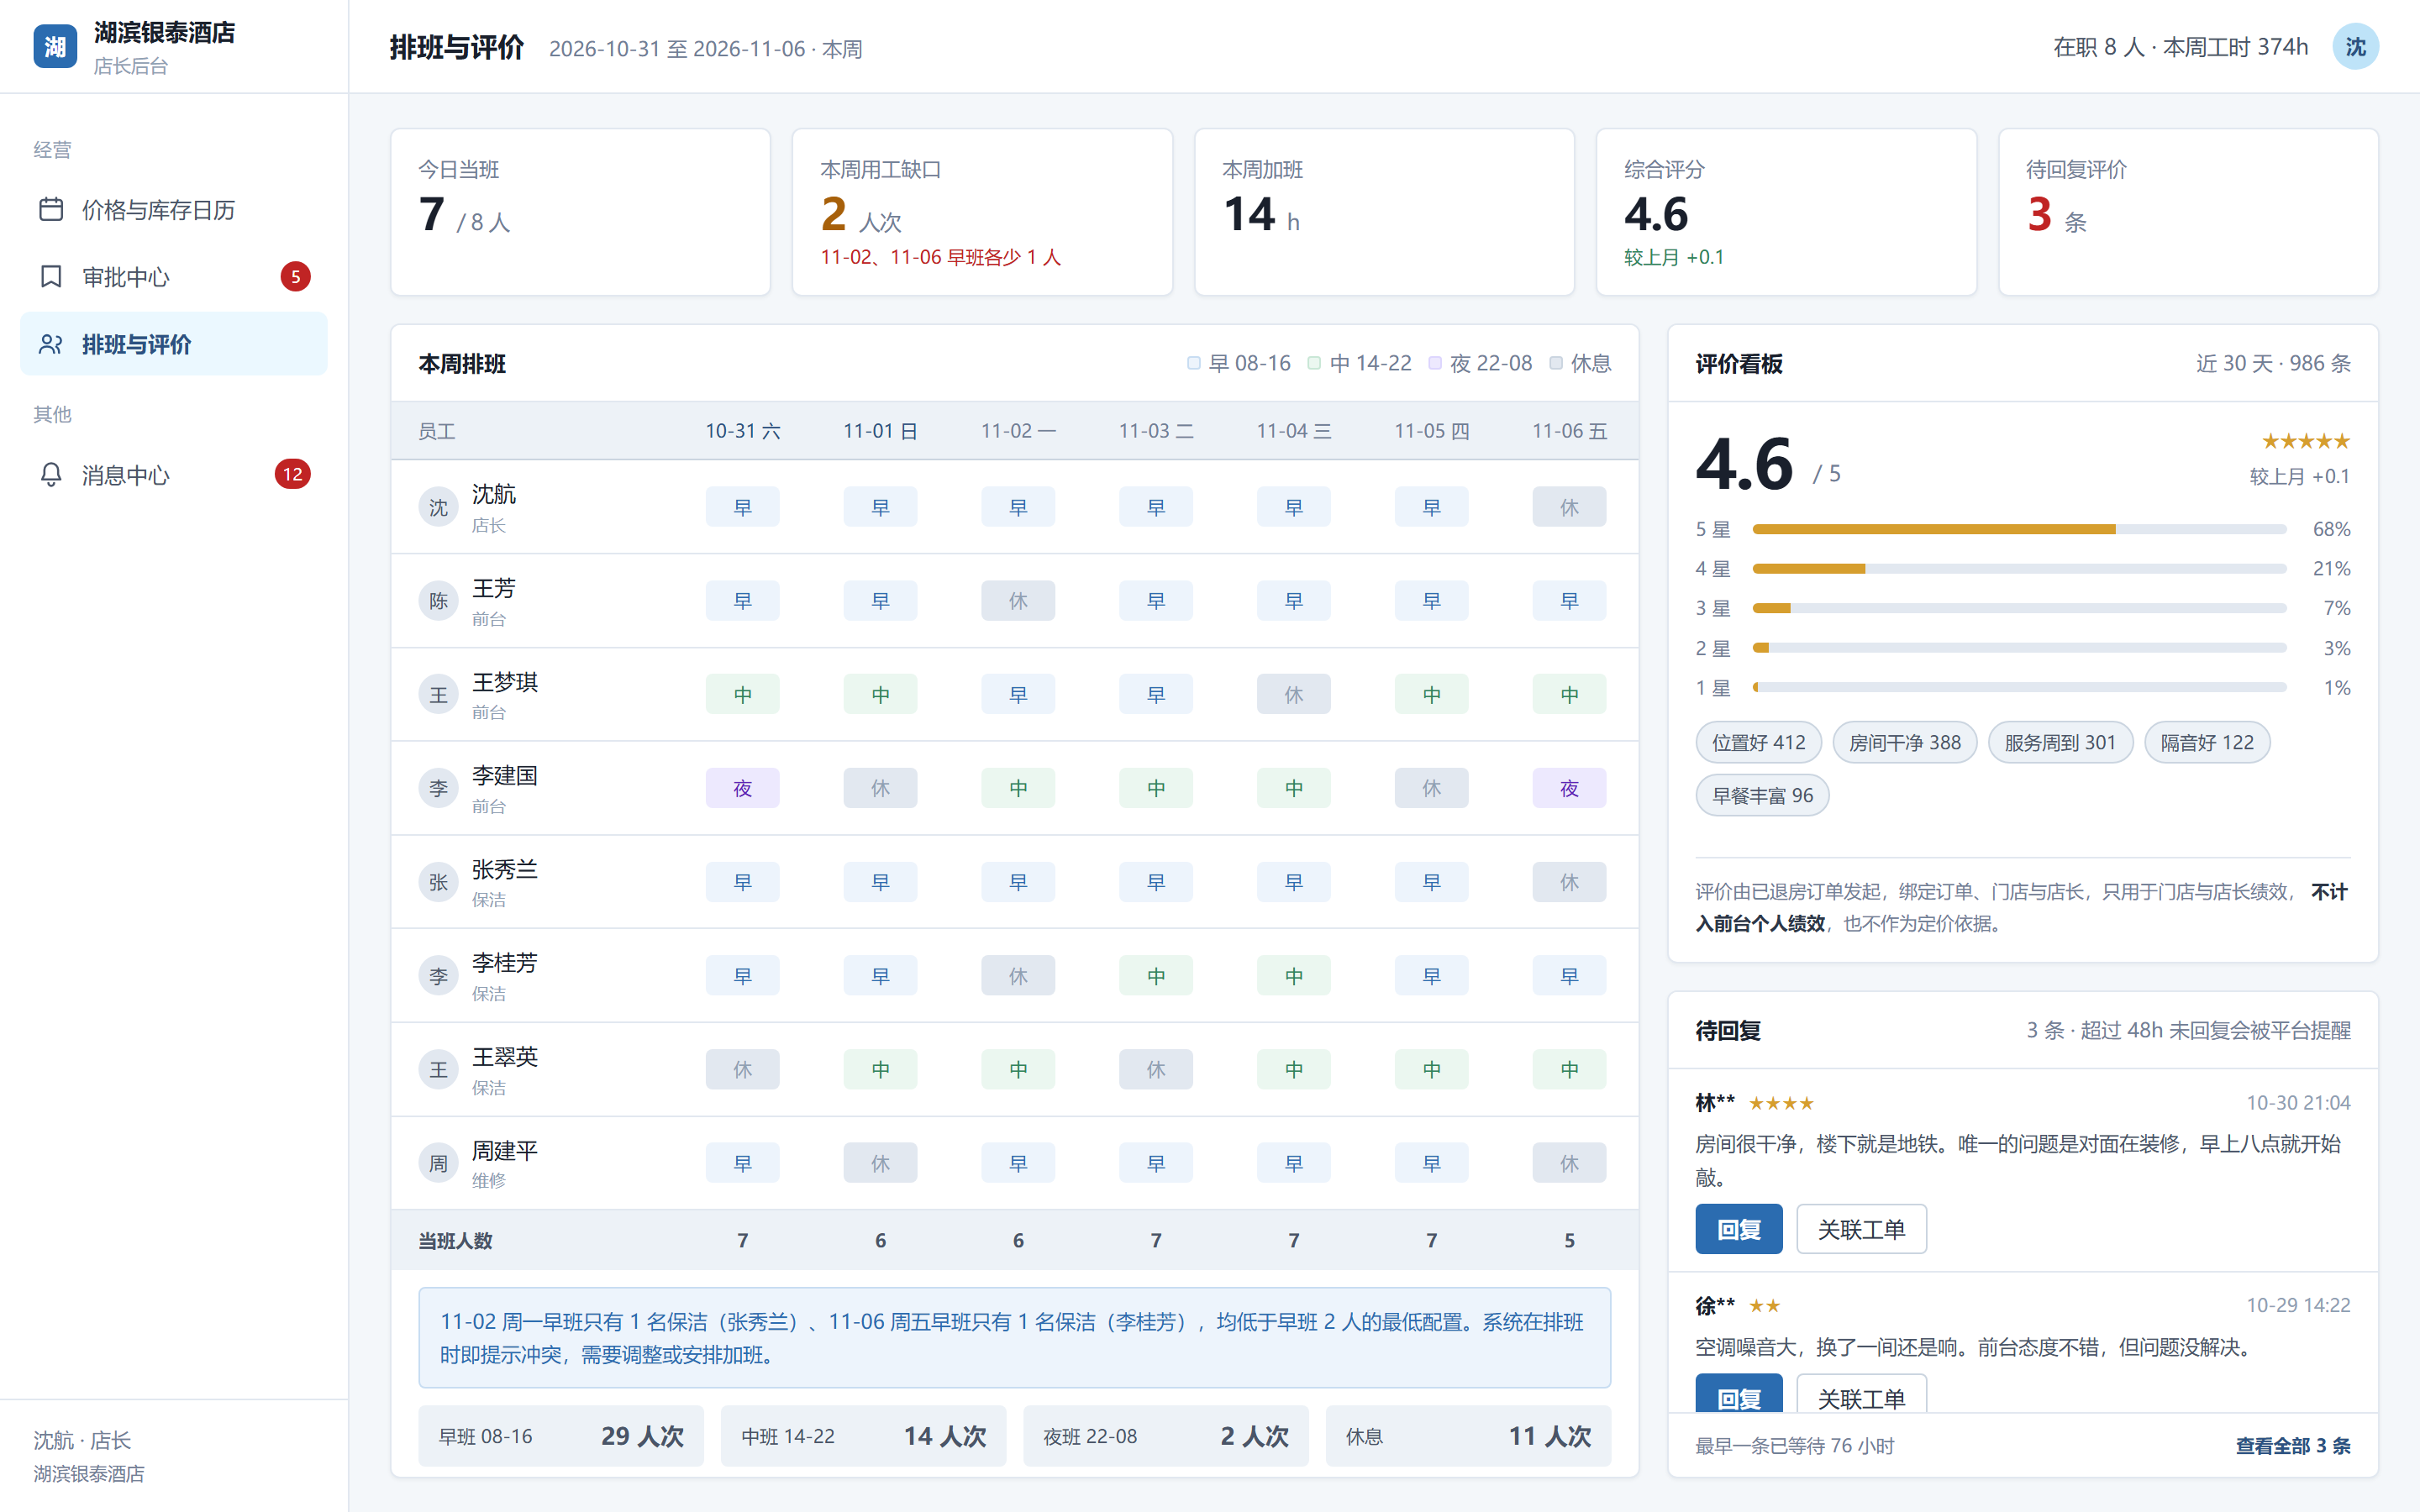
\includegraphics[width=\textwidth]{../UI界面/14_roster_review.png}
  \caption{排班与评价}
\end{subfigure}
\caption{店长端：排班与评价（14）}
\label{fig:ui_m2}
\end{figure}

\textbf{14 排班与评价。} 以周视图安排本店员工班次，标出缺岗日期；同屏展示综合评分和待回复评价。店长仅查看本店人员信息（REQ-026）。

\begin{figure}[htbp]
\centering
\begin{subfigure}[b]{0.95\textwidth}
  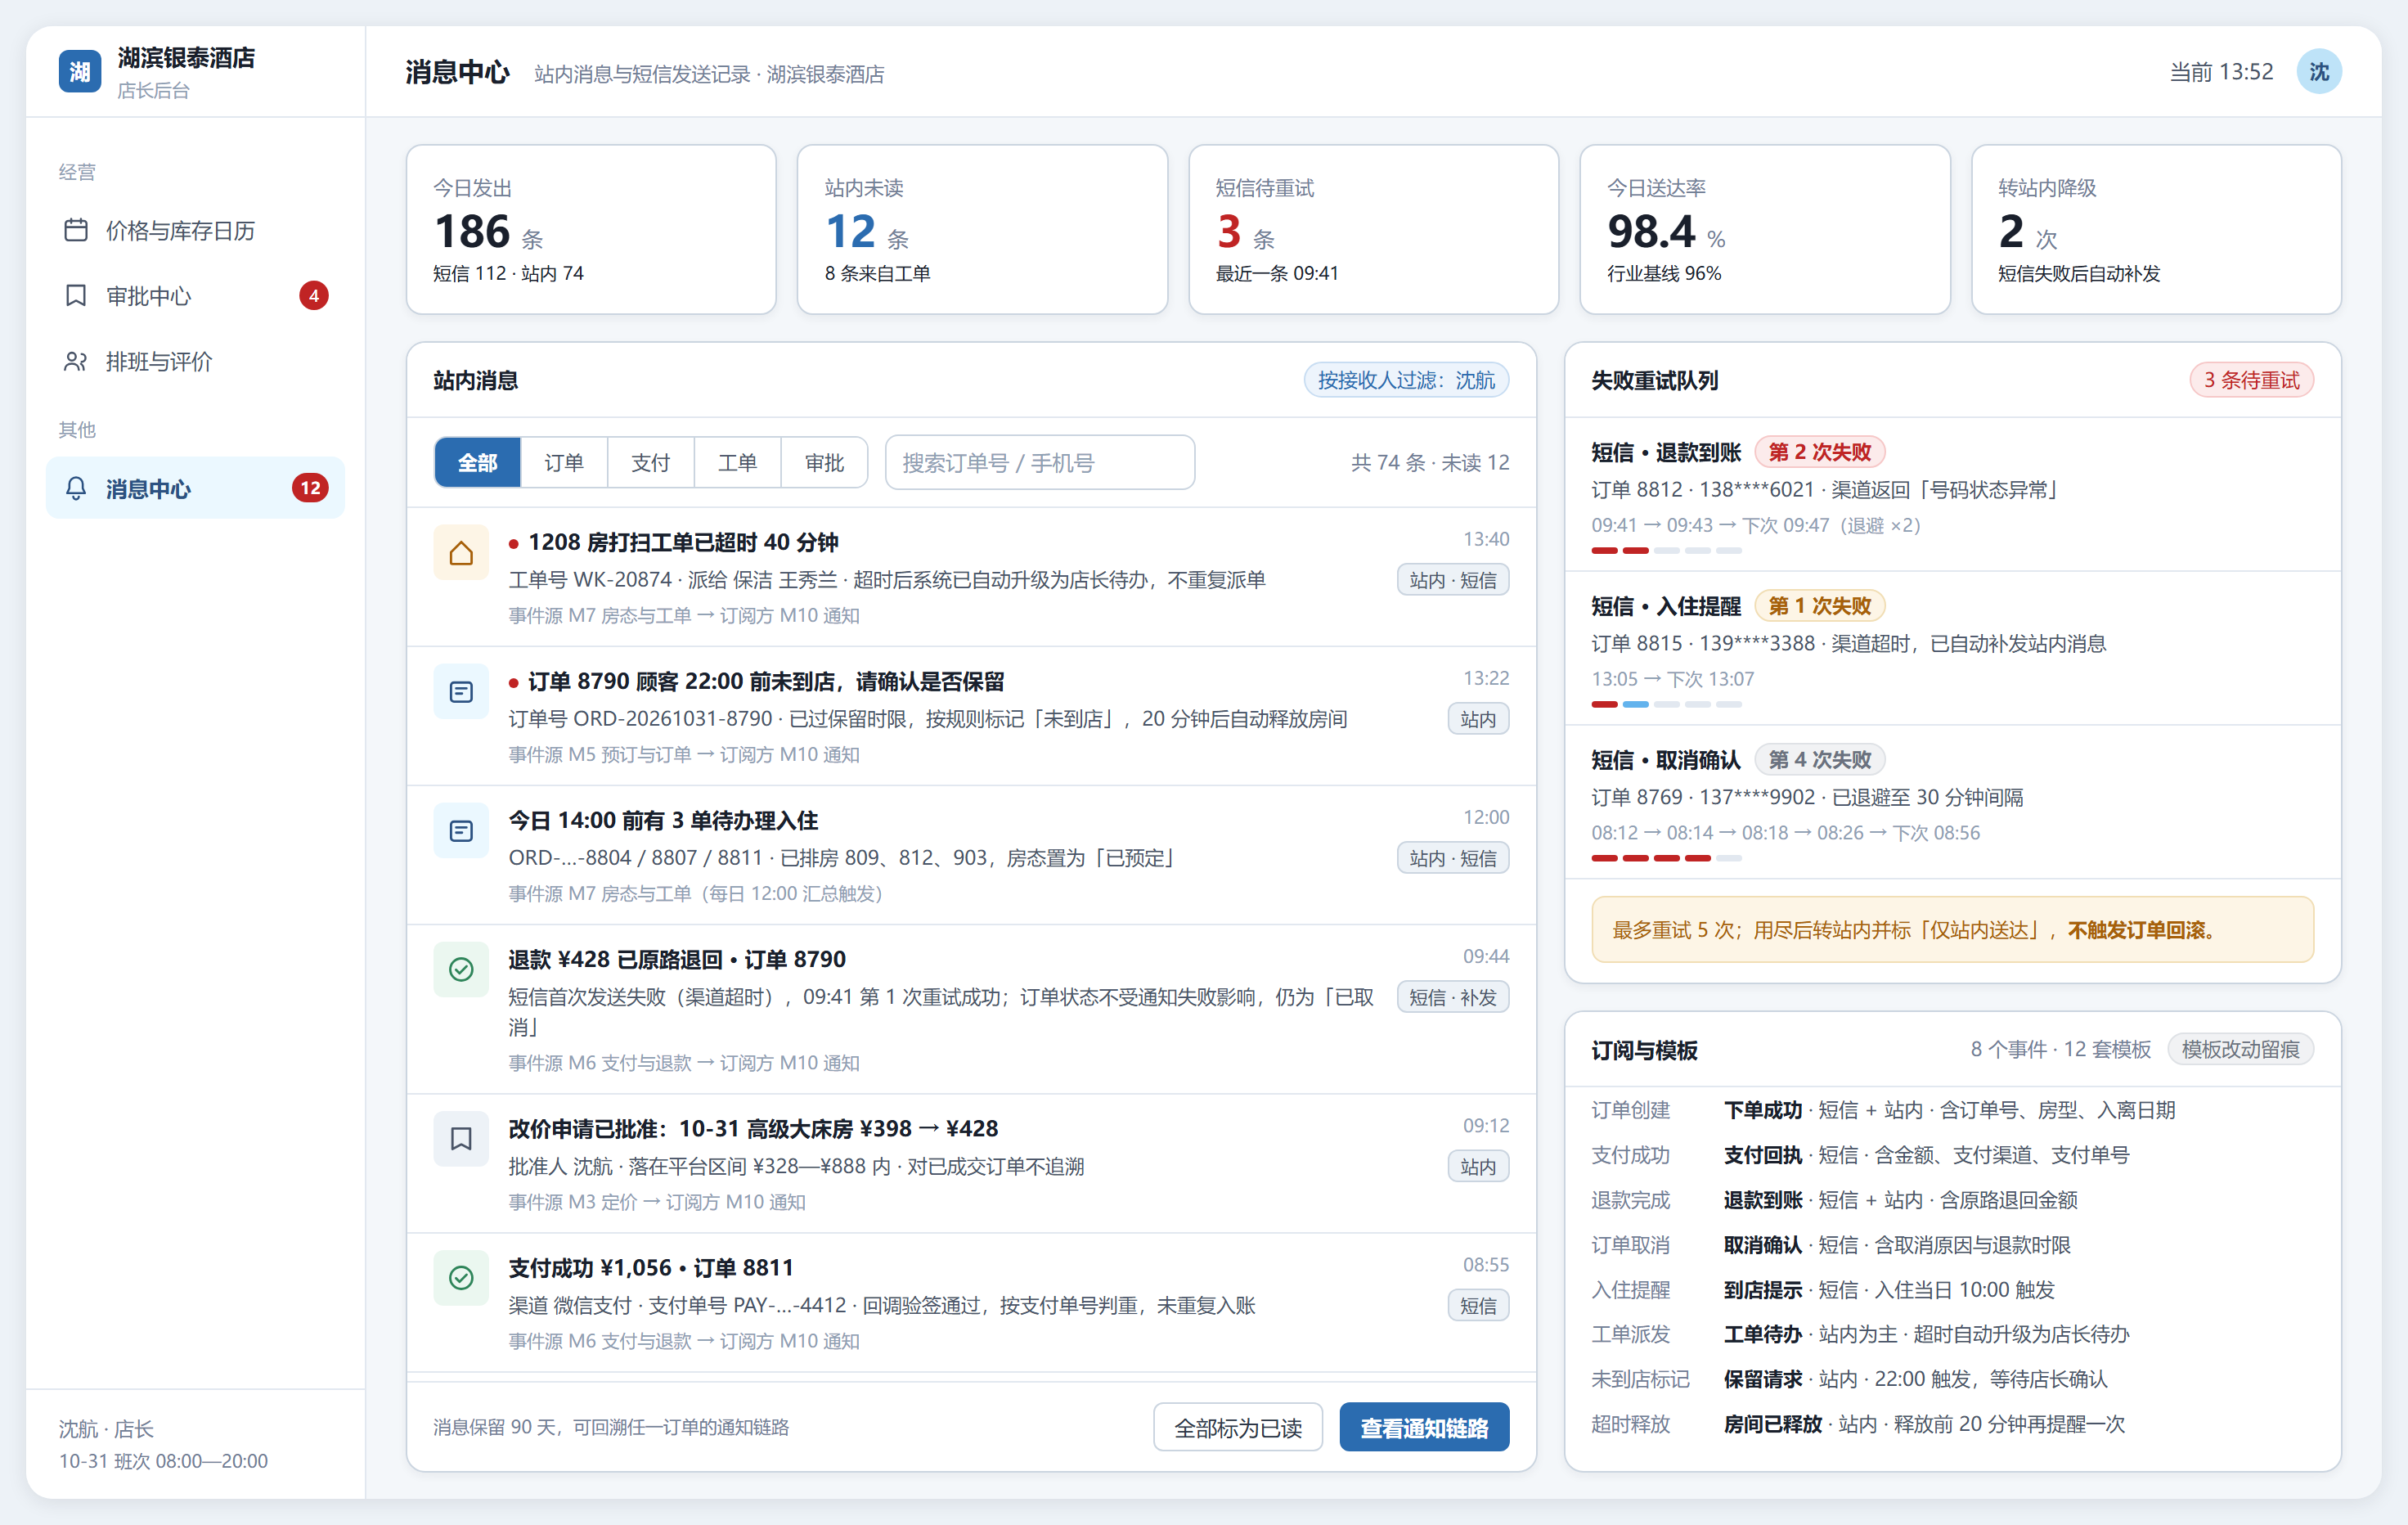
\includegraphics[width=\textwidth]{../UI界面/17_message_center.png}
  \caption{消息中心：站内消息、失败重试与订阅规则}
\end{subfigure}
\caption{店长端：消息中心（17）}
\label{fig:ui_m3}
\end{figure}

\textbf{17 消息中心。} 查询站内消息、短信发送状态与失败重试队列。通知最多重试五次，失败后转站内消息，不回滚订单；模板修改留痕（REQ-029）。

\subsection{平台端（4 屏，桌面后台）}

平台端提供跨店汇总、价格区间下发、人员调动和审计查询；不提供办理入住或修改房态入口（REQ-007）。

\begin{figure}[htbp]
\centering
\begin{subfigure}[b]{0.95\textwidth}
  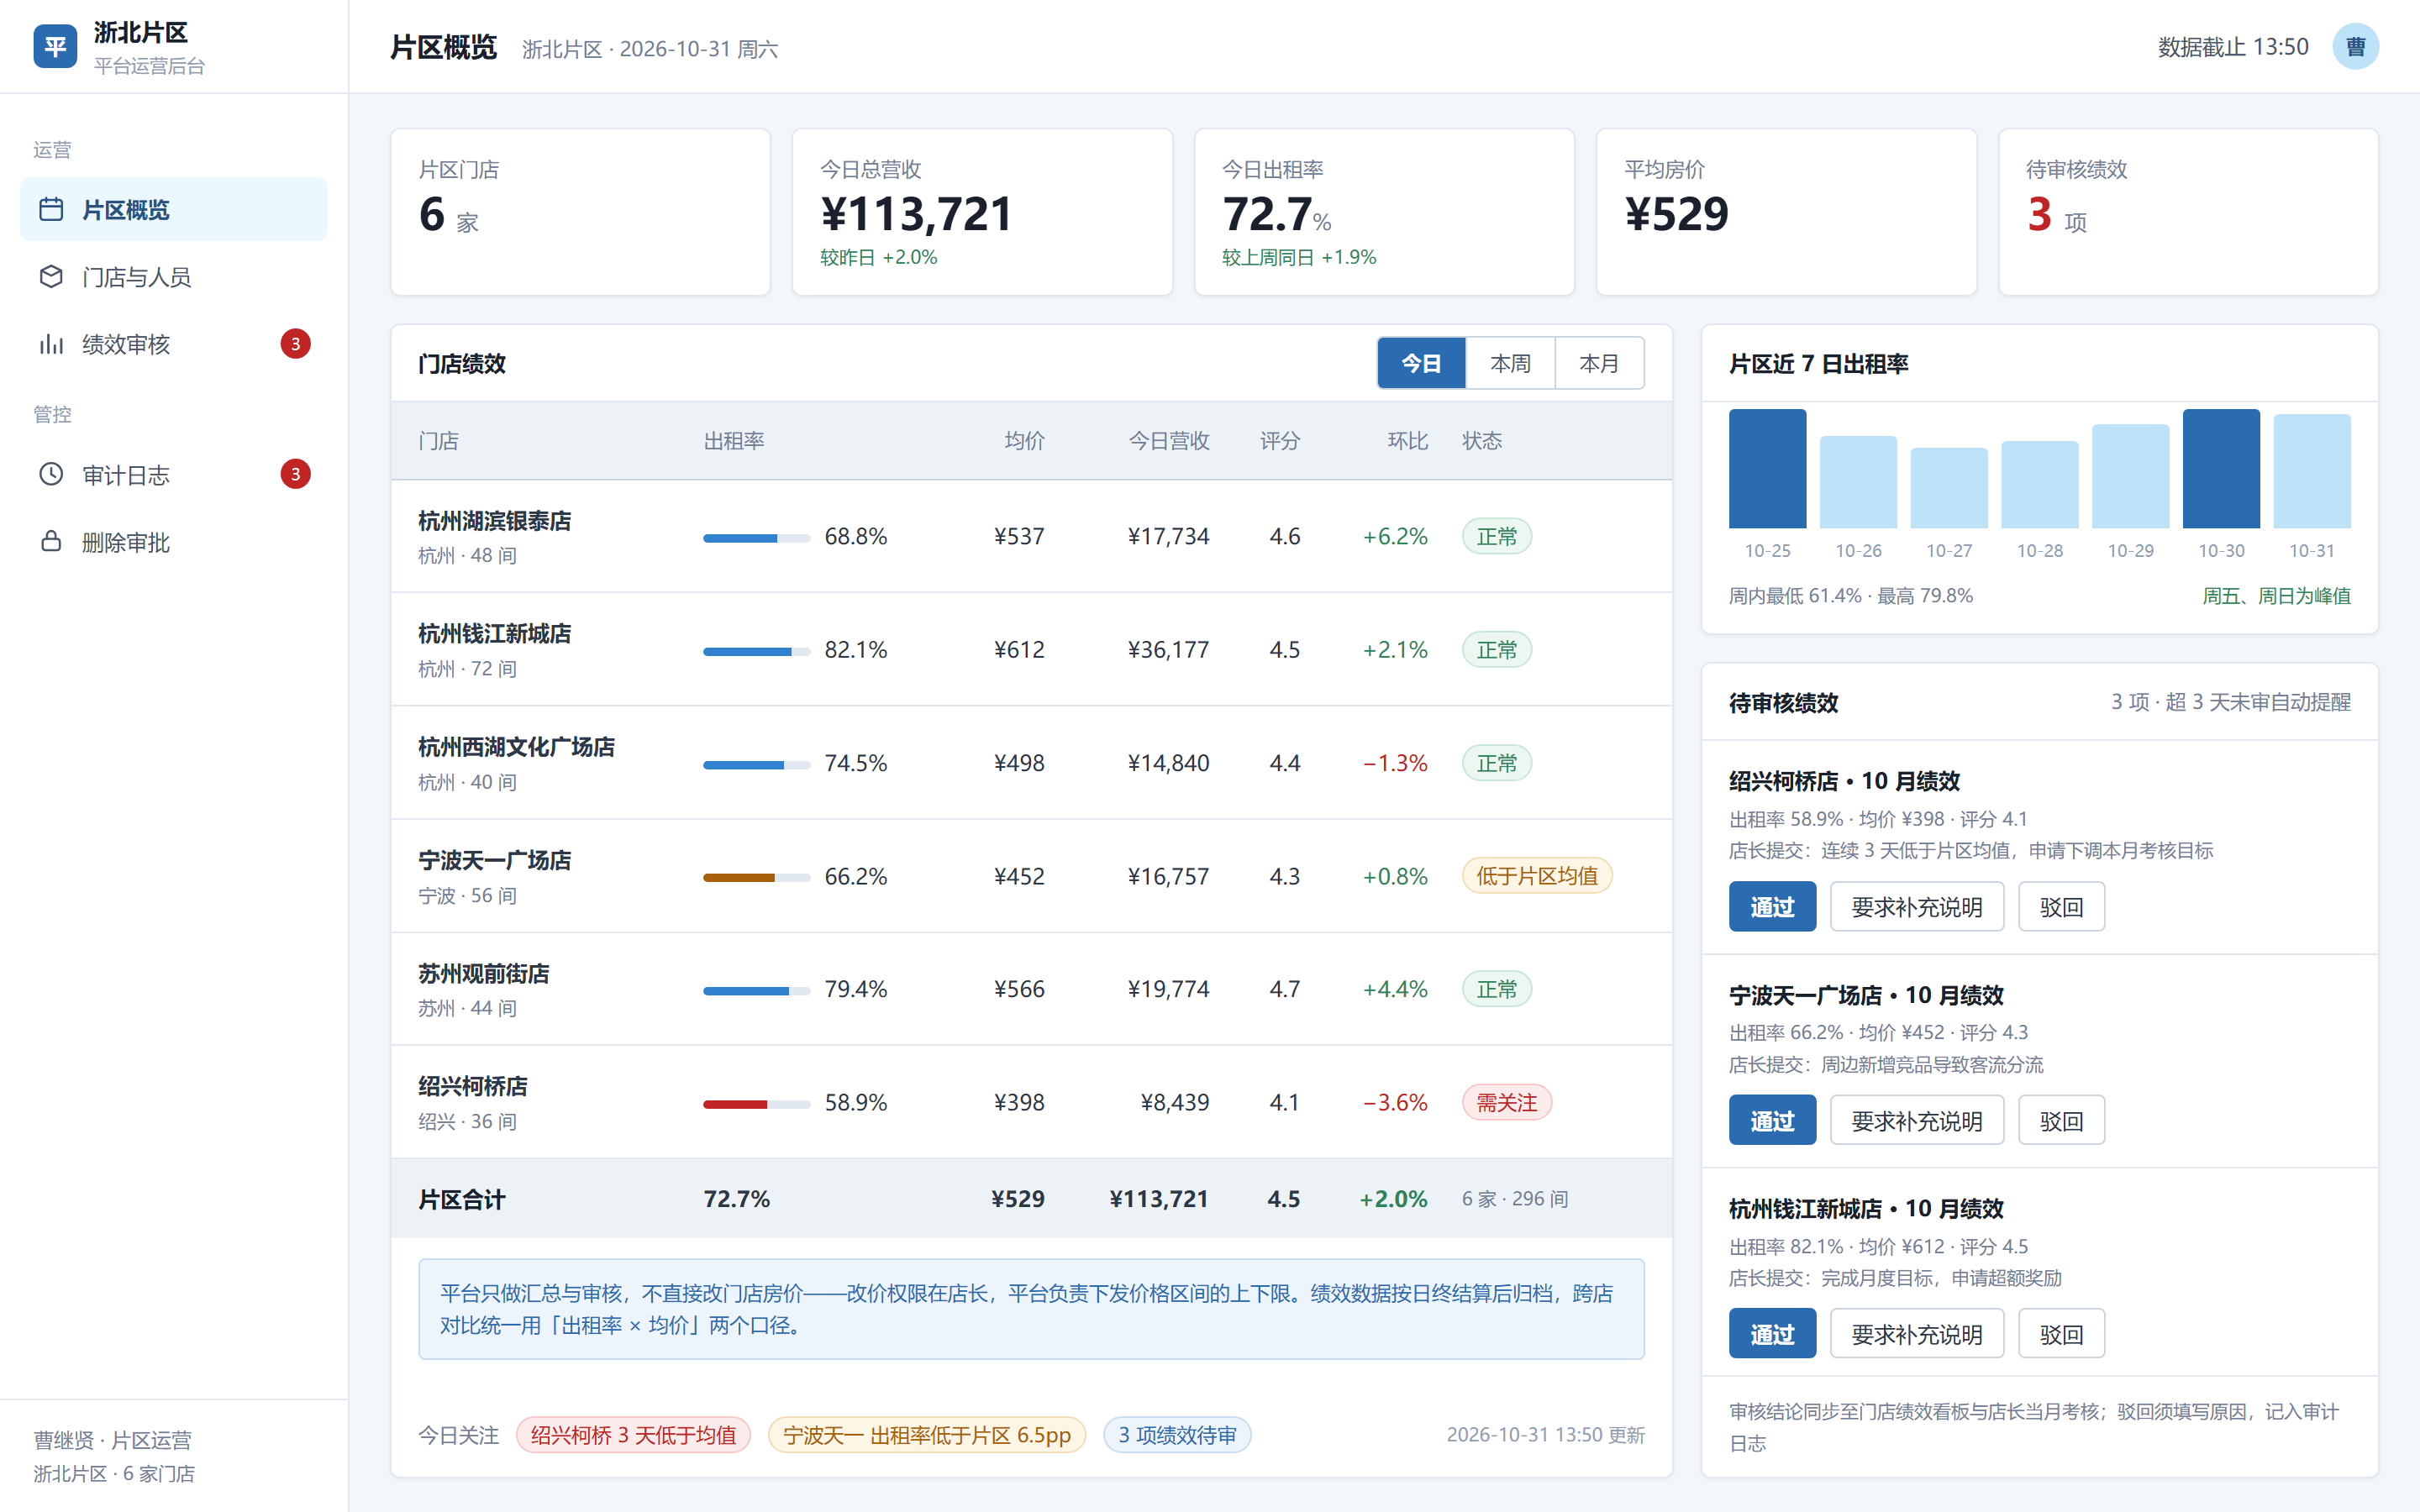
\includegraphics[width=\textwidth]{../UI界面/15_region_overview.png}
  \caption{片区概览与门店绩效}
\end{subfigure}\\[3pt]
\begin{subfigure}[b]{0.95\textwidth}
  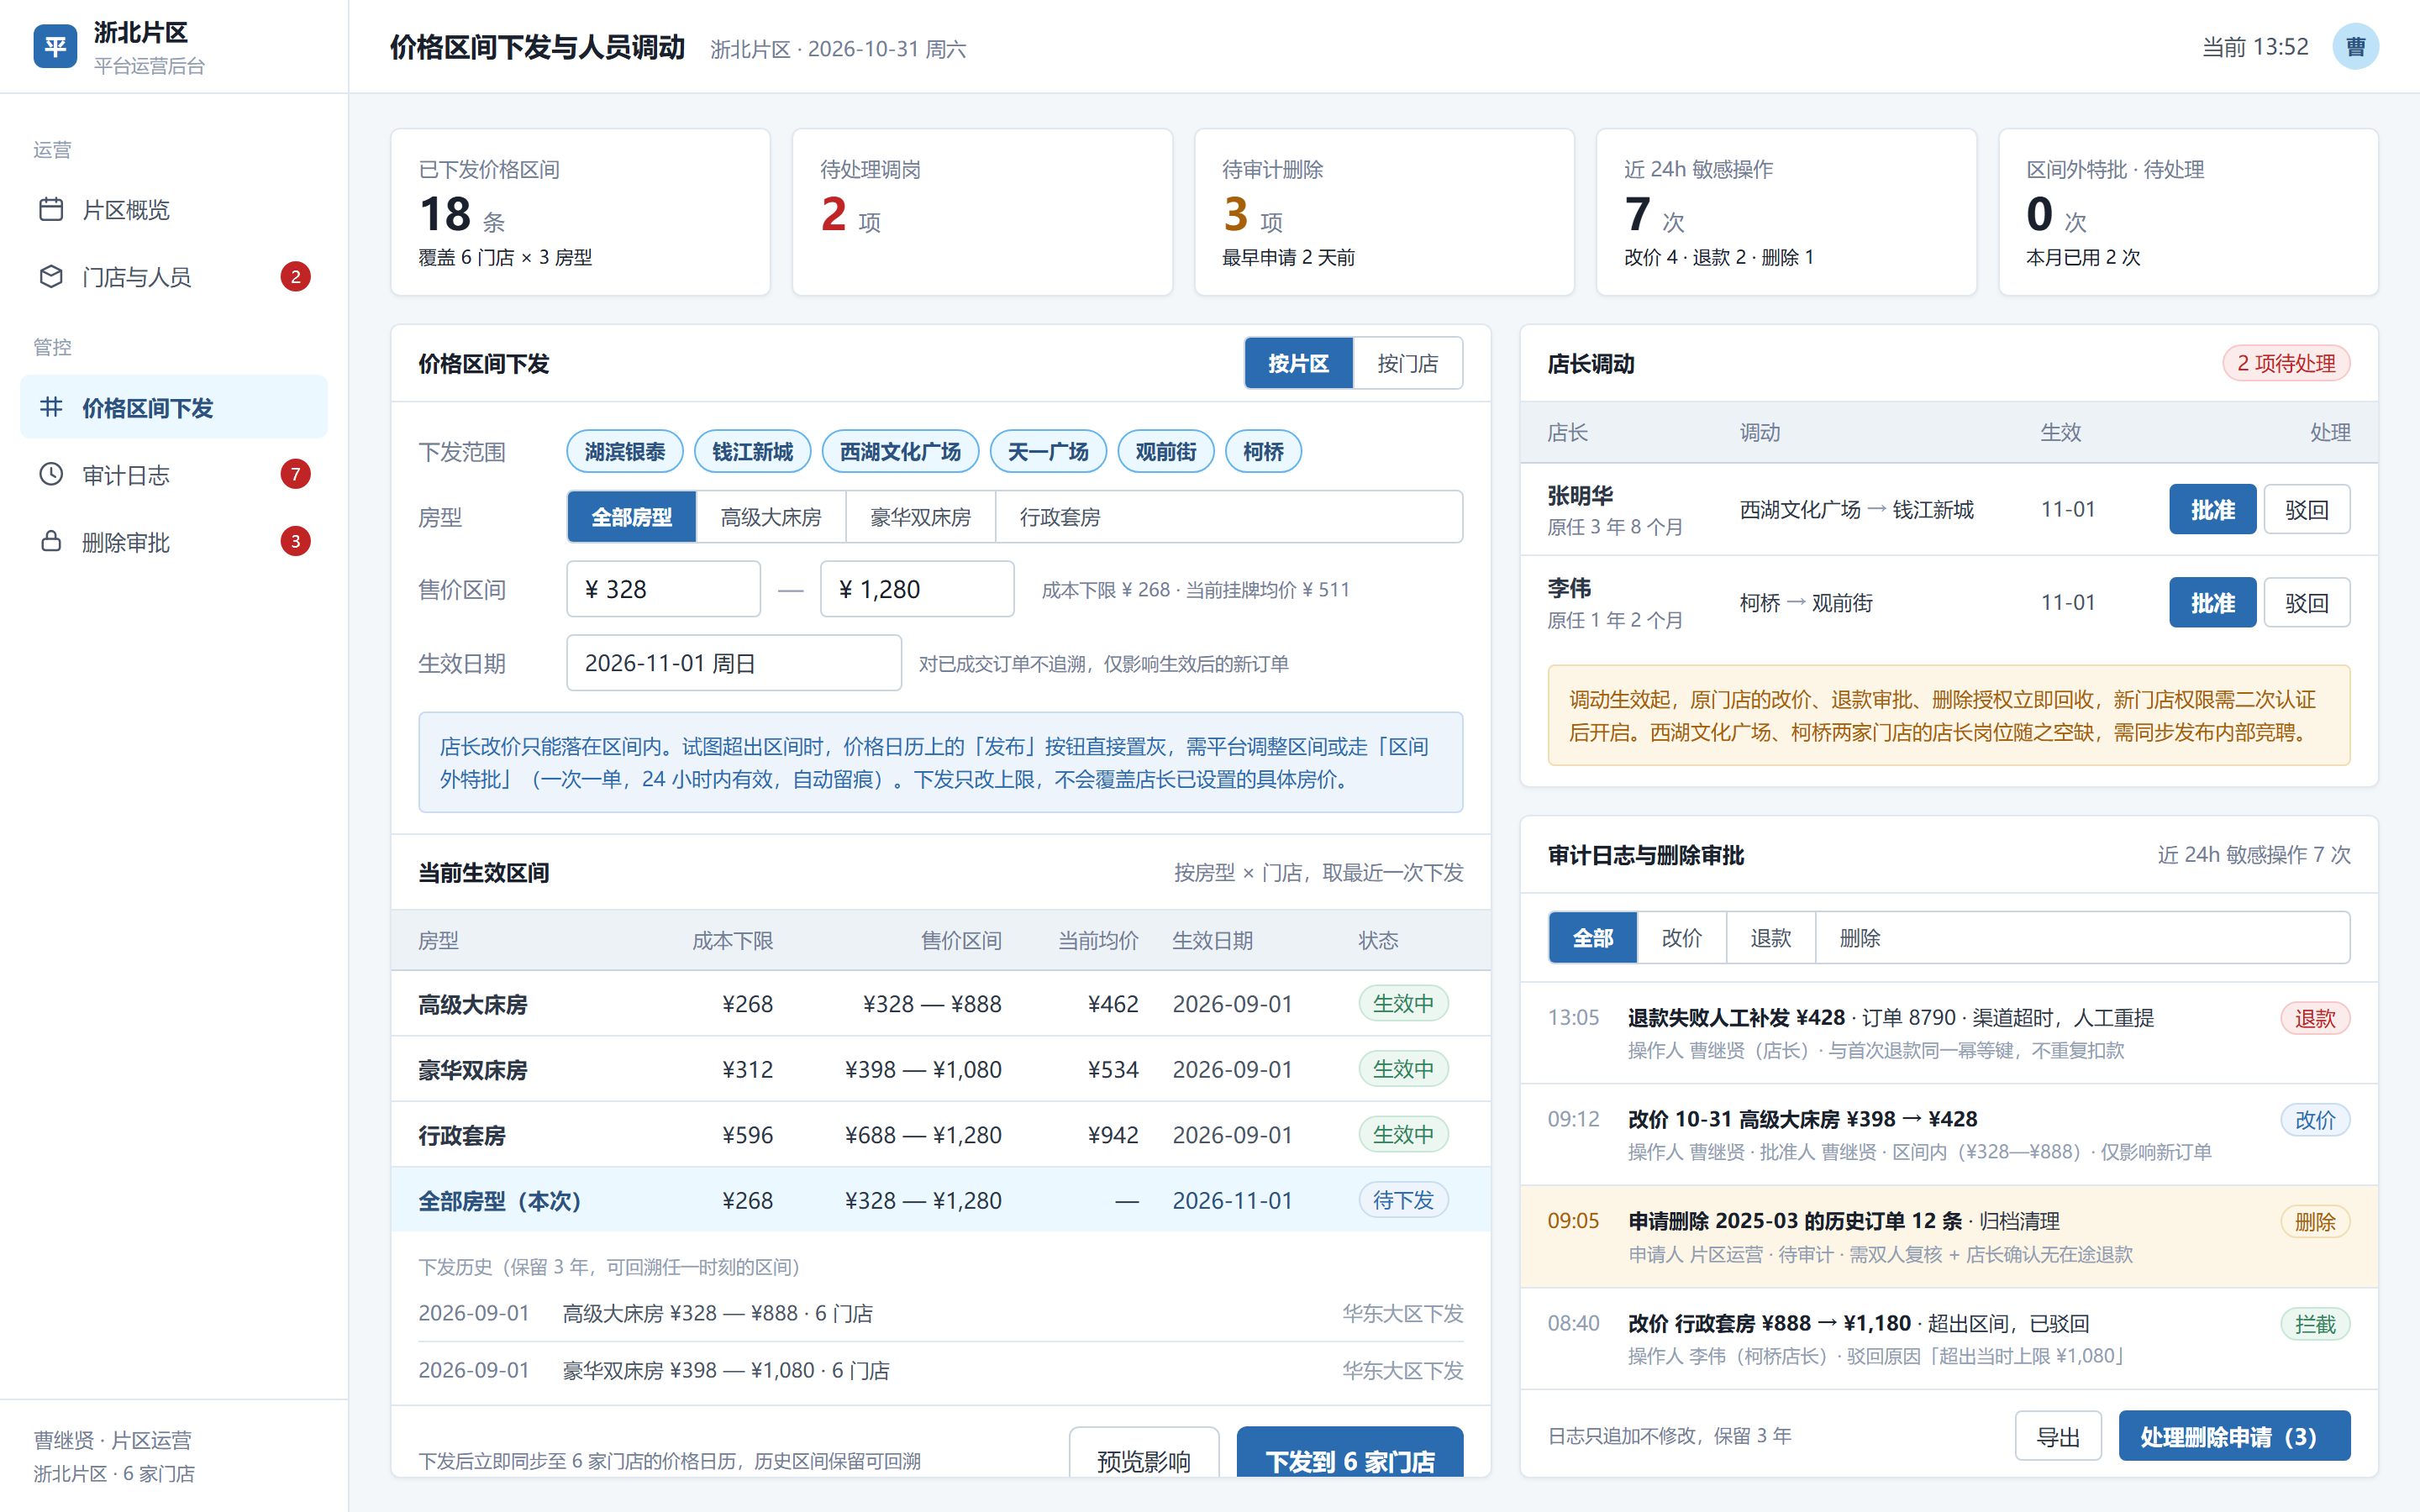
\includegraphics[width=\textwidth]{../UI界面/16_price_range_staffing.png}
  \caption{价格区间下发、人员调动与审计}
\end{subfigure}
\caption{平台端：片区概览与管控（15--16）}
\label{fig:ui_p}
\end{figure}

\textbf{15 片区概览与门店绩效。} 汇总六家门店的营收、出租率、均价和待审绩效；门店表展示各店评分及环比，右侧列出低于片区均值的门店。示例片区营收 ¥113,721、加权出租率 72.7\%。平台端只审核绩效，不直接修改门店房价（REQ-007）。

\textbf{16 价格区间下发、人员调动与审计。} 平台选择门店、房型、生效日期和价格区间，下发后只约束新订单，不改历史成交价（REQ-023）。同屏处理店长调动并查看敏感操作摘要；调动生效时回收原门店权限（REQ-007、REQ-014）。

\begin{figure}[htbp]
\centering
\begin{subfigure}[b]{0.95\textwidth}
  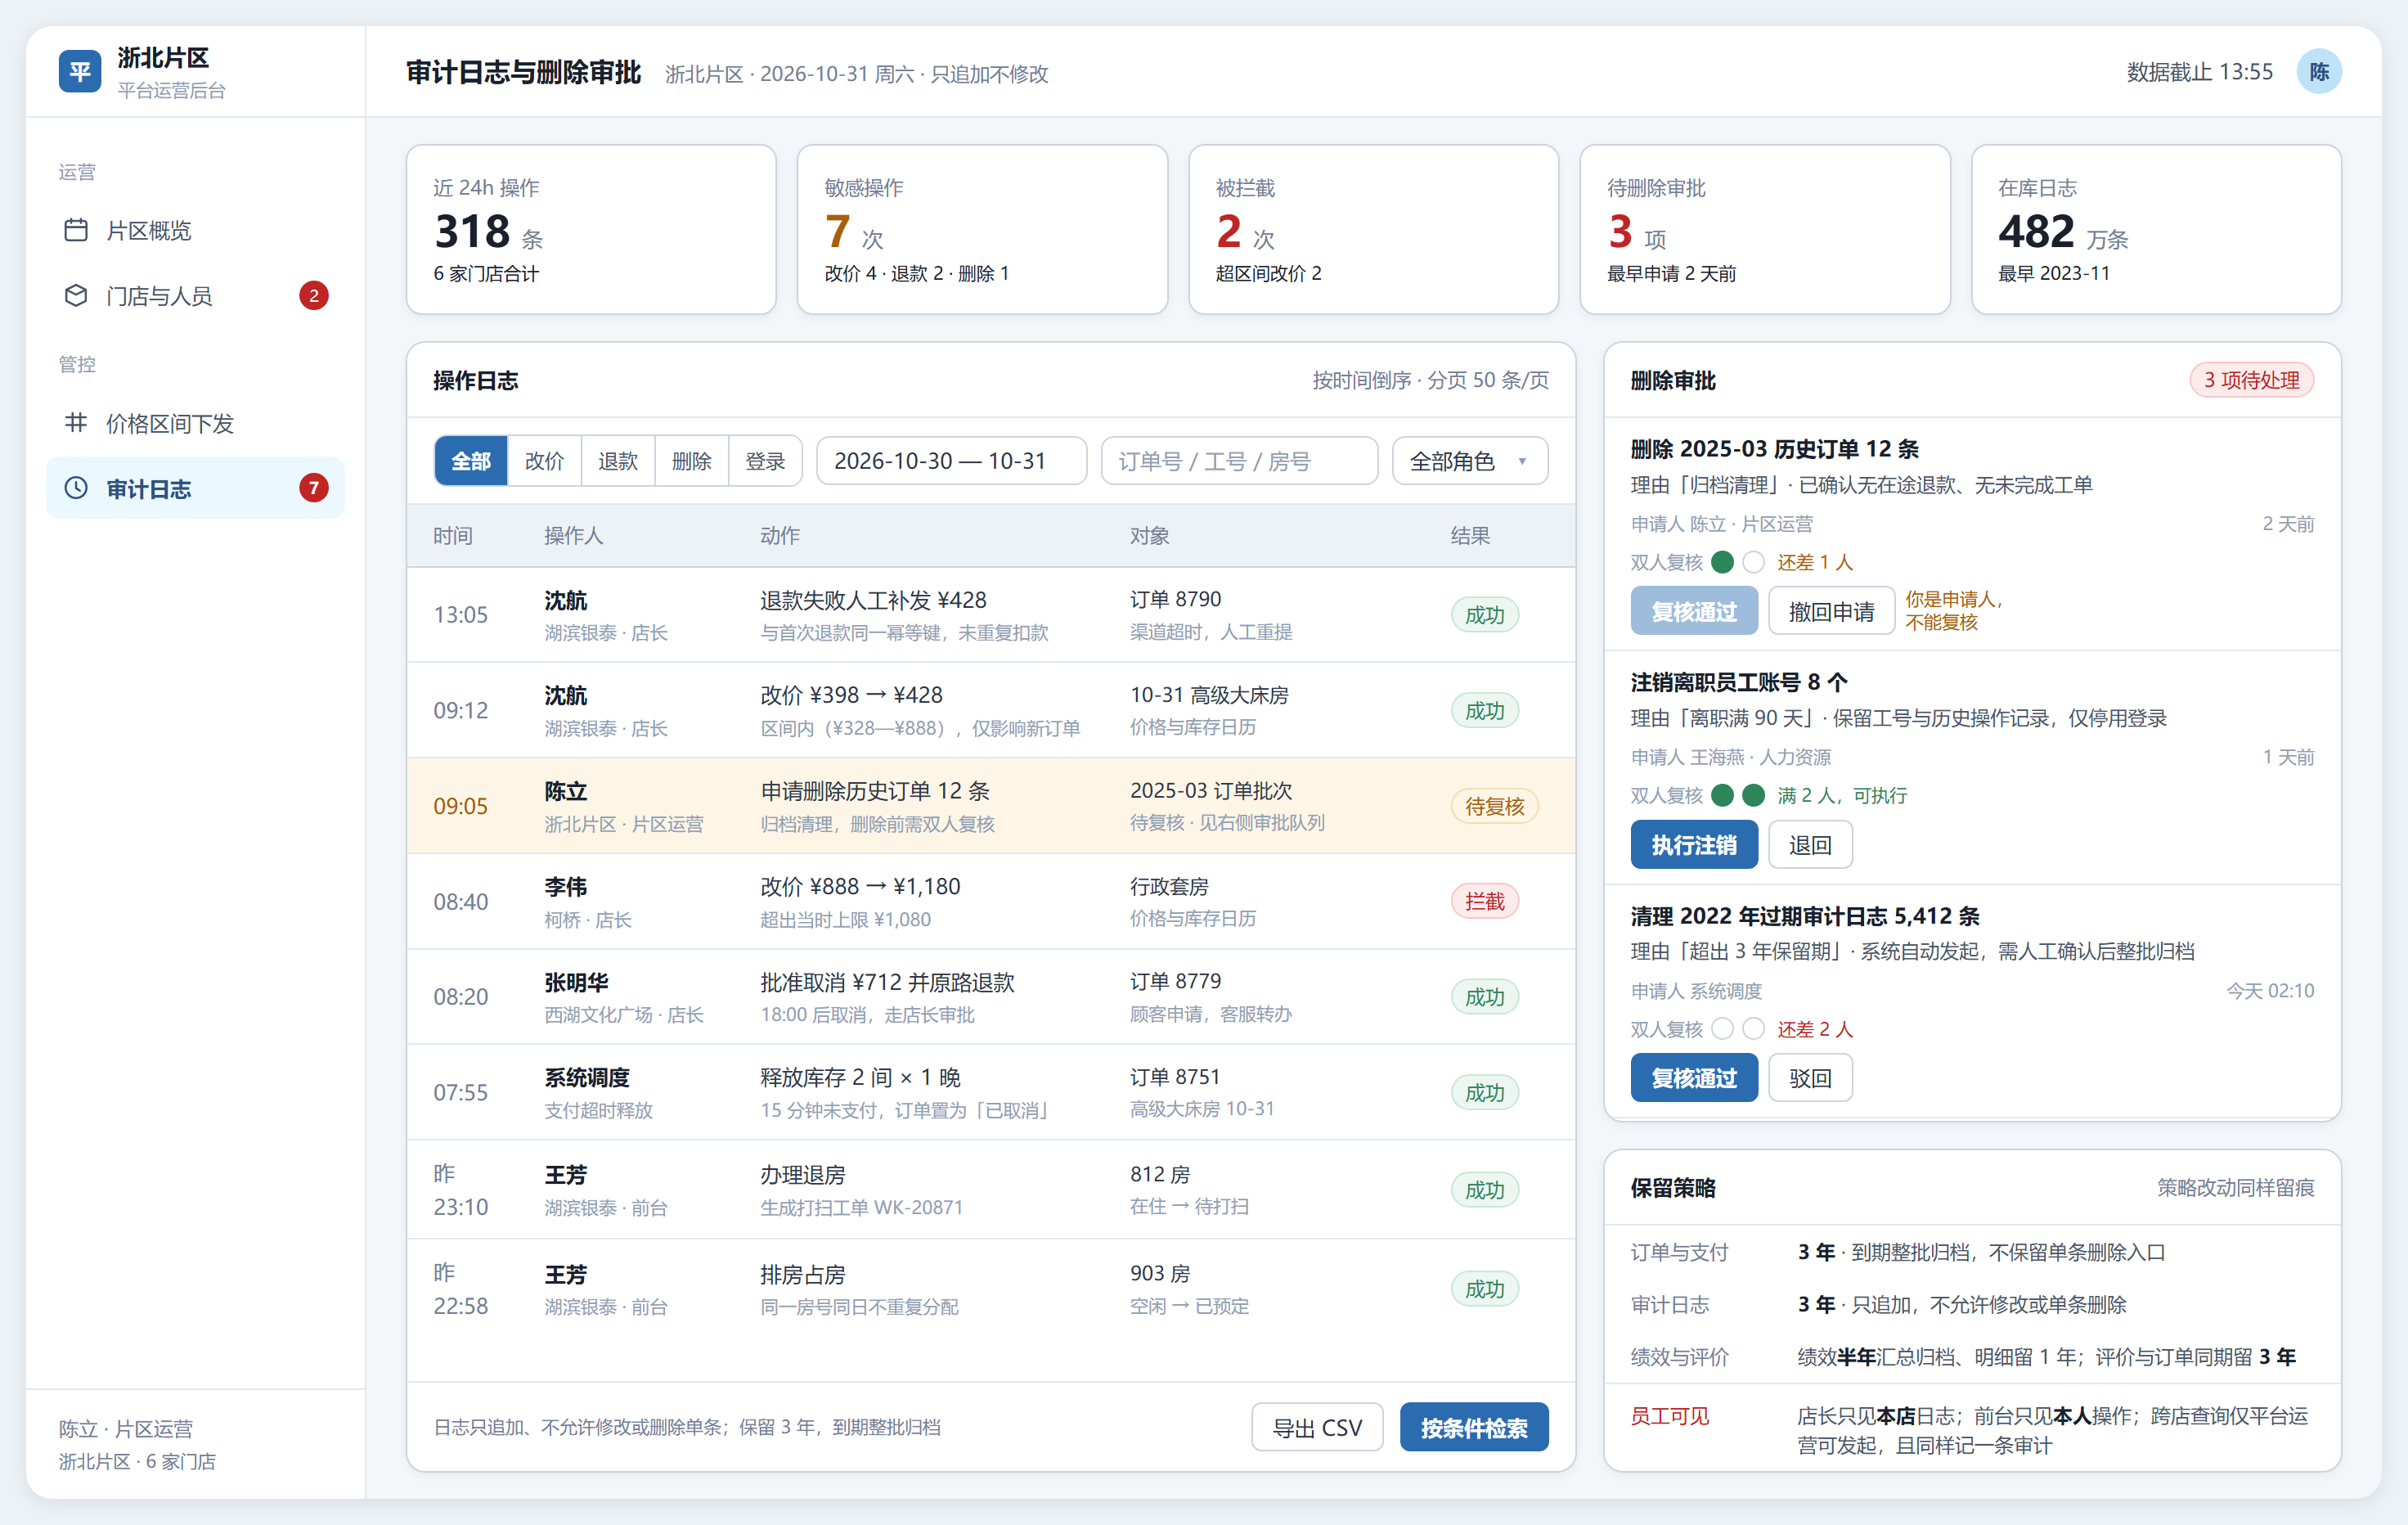
\includegraphics[width=\textwidth]{../UI界面/18_audit_log.png}
  \caption{审计日志与删除审批}
\end{subfigure}\\[3pt]
\begin{subfigure}[b]{0.95\textwidth}
  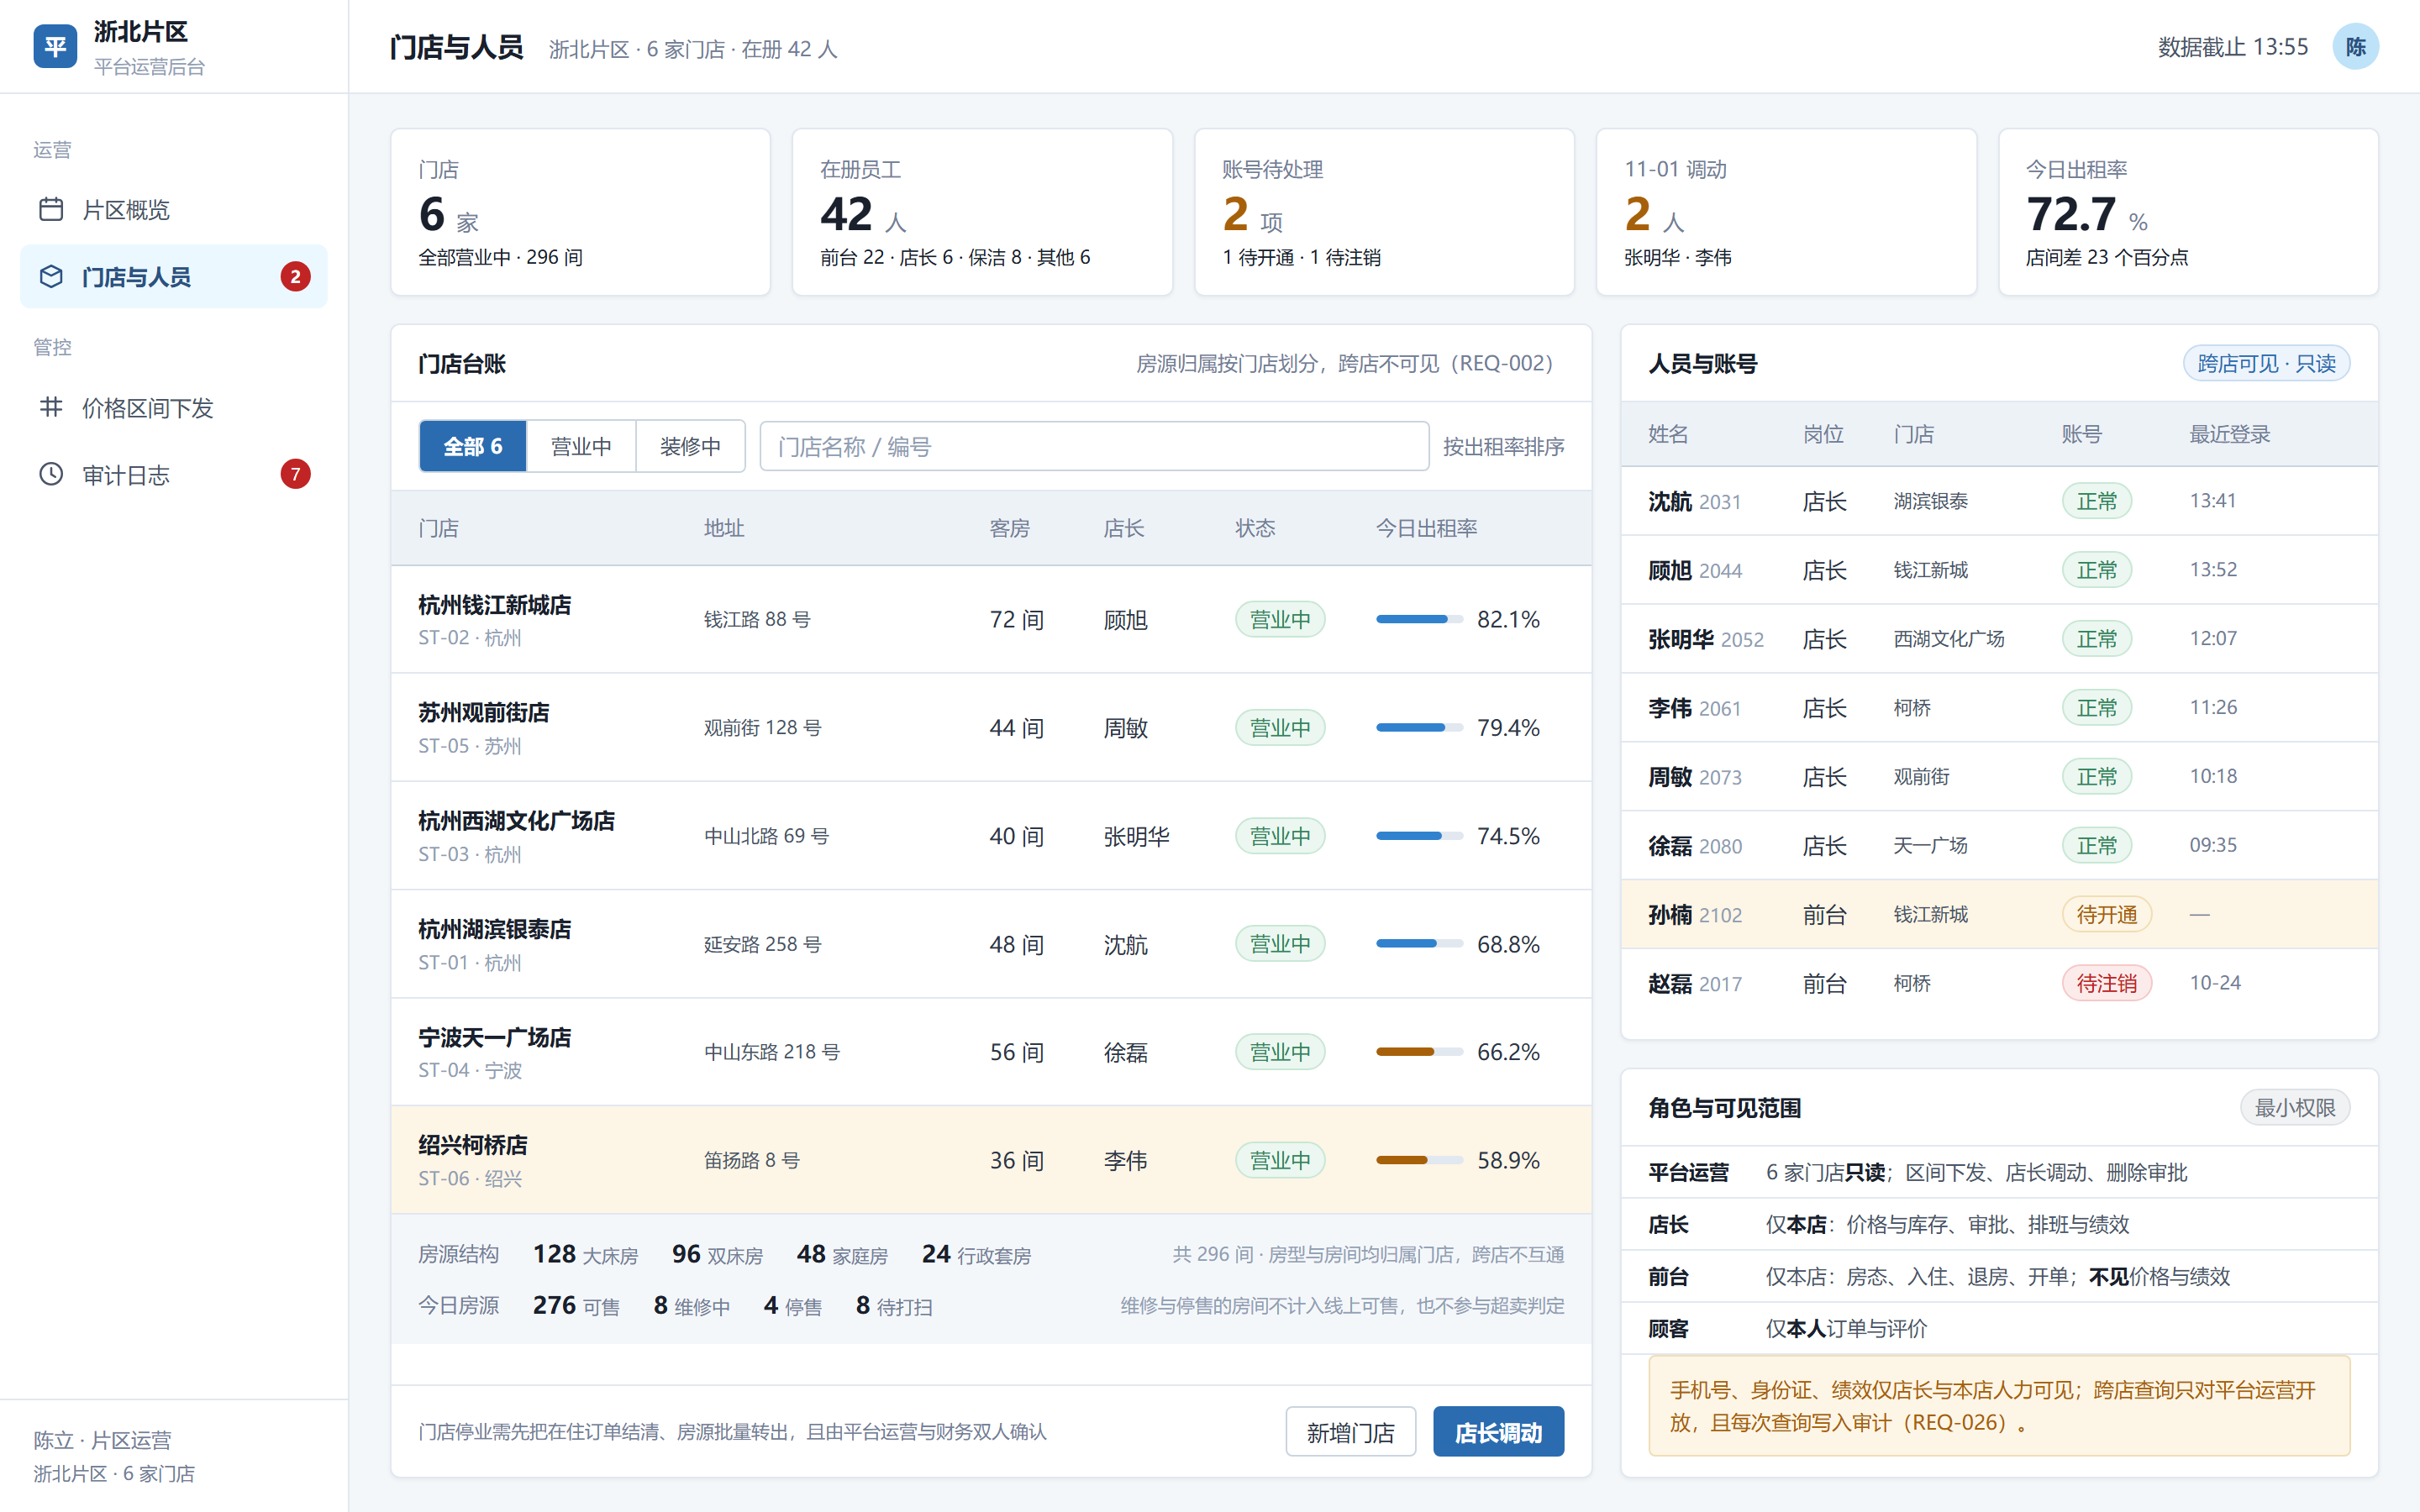
\includegraphics[width=\textwidth]{../UI界面/19_store_staff.png}
  \caption{门店与人员}
\end{subfigure}
\caption{平台端：审计与组织（18--19）}
\label{fig:ui_p2}
\end{figure}

\textbf{18 审计日志与删除审批。} 日志按时间列出操作人、动作、对象及结果，包含被拦截操作和系统定时任务；记录只追加、保留三年。删除审批展示复核进度，要求执行人与申请人不同；跨店查询同样留痕（REQ-014、REQ-026、REQ-030）。

\textbf{19 门店与人员。} 展示六家门店的房量、出租率、负责人及员工账号状态；调动在生效日前标为待生效，离职账号停用但保留历史操作。页面按角色展示可见范围，店长限本店、前台限本店业务、顾客限本人记录（REQ-001、REQ-026）。

\subsection{界面—模块—需求对照}

下表列出 19 屏界面对应的主要模块与需求。

{\tabfont
\begin{xltabular}{\textwidth}{@{}L{0.6cm}L{3.3cm}L{2.4cm}X@{}}
\caption{界面、模块与需求的对应关系}\label{tab:ui_map}\\
\toprule
\# & 界面 & 主要模块 & 落地的需求 \\
\midrule
\endfirsthead
\toprule
\# & 界面 & 主要模块 & 落地的需求 \\
\midrule
\endhead
\midrule
\multicolumn{4}{r}{\zihao{6}续下页}\\
\endfoot
\bottomrule
\endlastfoot
01 & 首页与搜索 & M2、M4 & REQ-002 查询；REQ-019 范围约束 \\
02 & 搜索结果 & M2、M4 & REQ-002；REQ-013 按日期逐晚的余量 \\
03 & 酒店详情与房型 & M2、M3、M4 & REQ-013 可订量取最小；REQ-023 明码标价 \\
04 & 订单确认 & M3、M5 & REQ-020 倒计时；REQ-023 价格快照；REQ-021 取消政策 \\
05 & 支付 & M6、M5 & REQ-020 超时释放；REQ-021 取消截止；REQ-028 一致性 \\
06 & 我的订单 & M5 & REQ-008 六态筛选；REQ-031 改期入口；REQ-003 评价入口 \\
07 & 评价提交 & M8 & REQ-003 仅已退房可评、一单一评 \\
08 & 房态看板 & M7、M2 & REQ-005 六种房态；REQ-022 超时未退；REQ-034 维修与可售 \\
09 & 排房与入住 & M7、M5 & REQ-018 三步入住；REQ-004 入住；REQ-024 排房占房 \\
10 & 退房与打扫 & M7 & REQ-003 退房；REQ-022 逾期；REQ-025 打扫工单 \\
11 & 线下开单 & M4、M5 & REQ-033 上限与线下保留；REQ-032 多晚次 \\
12 & 价格与库存日历 & M3、M4 & REQ-006 店长设价；REQ-033 上限；REQ-013 逐晚库存 \\
13 & 审批中心 & M3、M4、M5、M9 & REQ-014 留痕；REQ-021 取消审批；REQ-025 工单；REQ-034 维修 \\
14 & 排班与评价 & M8 & REQ-026 员工信息范围；REQ-003 评价；REQ-007 绩效汇总 \\
15 & 片区概览与绩效 & M8、M1 & REQ-007 平台管理；REQ-026 可见范围 \\
16 & 价格区间与人员调动 & M3、M1、M9 & REQ-007；REQ-030 删除审批；REQ-009 幂等退款留痕 \\
17 & 消息中心 & M10、M5 & REQ-029 通知失败不回滚；REQ-010 事件订阅 \\
18 & 审计日志与删除审批 & M9 & REQ-030 双人复核与回避；REQ-014 操作留痕；REQ-026 可见范围 \\
19 & 门店与人员 & M1、M2 & REQ-001 账号与权限；REQ-002 门店归属；REQ-026 员工信息范围 \\
\end{xltabular}
}

REQ-035、REQ-036 在实验一尚未确认，因此界面未设计对应流程。性能、可靠性等全局约束不单独设置界面；权限通过各端可见菜单和操作范围体现。
